\chapter{Discrete Nonlinear Model Development for Urea SCR-ASC Dynamics}

One of the fundamental assumptions in the diesel engine SCR-ASC modelling, CSTR, reverts the causality in the reaction
rate constants, when the model order is reduced by considering a single cell. The present work circumvents the problem
by discarding the CSTR assumption and modelling the time evolution of the sensor signals when a "plug" or "parcel" of
the exhaust gasses flows through the chamber.

Such a time evolution introduces constraints on the model due to sampling limitations. To capture the transient
dynamics, the sampling time should be significantly smaller than the "residence time" of the reactants inside the
SCR-ASC chamber. If that is not the case as is the situation with the present available test and truck data, time integrated states assuming zero-order holds during the transients need to be introduced into the model and the input-output model can be derived from the resulting state-space model.

The modelling approach involves following the evolution of the measurement signals at the input and the output of the
system. As the plug of fluid flows through the chamber, these measurements can be correlated based on the conservation
of moles within the fluid plug.


\section{Ammonia Adsorption/Desorption Process Dynamics}
\begin{figure}[h!]
    \centering
    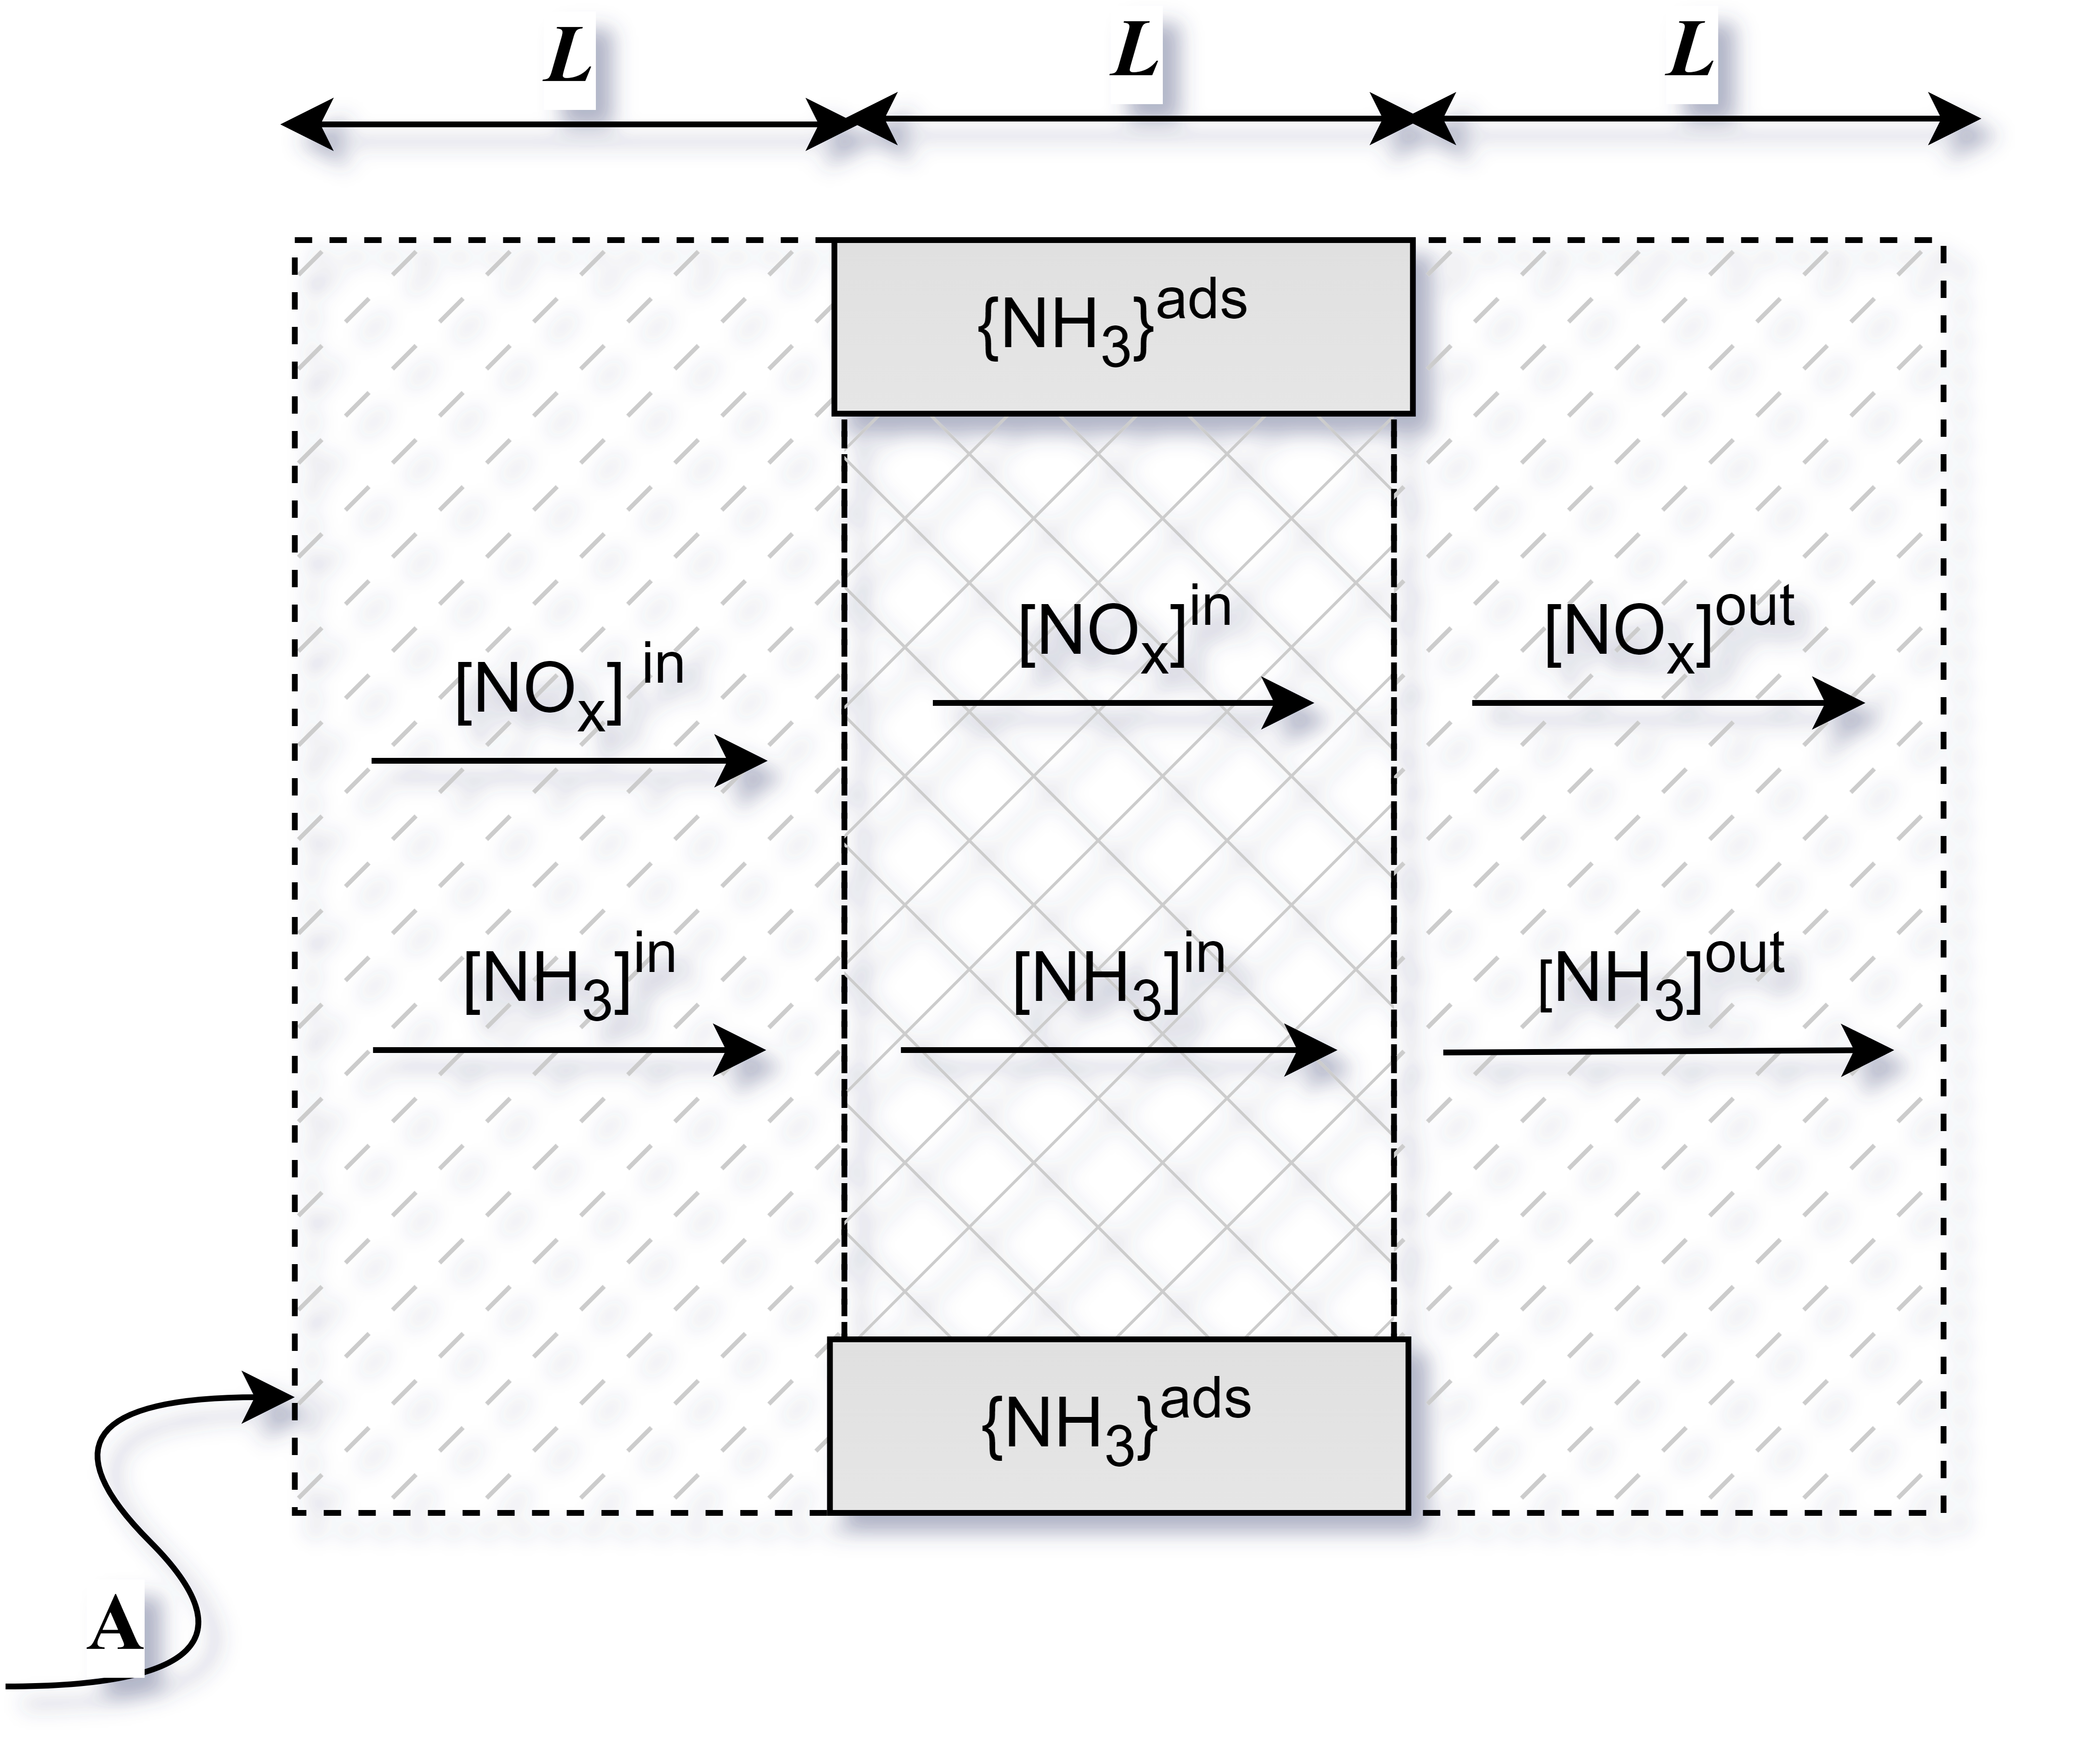
\includegraphics[width=0.5\textwidth]{Part3/figs/plug_flow_discrete.png}
    \caption{Discrete plug-flow reactor model}
    \label{fig:plug_flow_discrete}
\end{figure}
%===
The ammonia adsorption/desorption process dynamics involve all the three above-mentioned reactions. The gaseous ammonia
that enters the catalyst chamber gets adsorbed onto the free sites on the catalyst surface at a rate proportional to the
volumetric concentration of the gaseous ammonia and the surface concentration of the free sites. The adsorbed ammonia
then either reacts with the gaseous $NO_x$ (Eiley-Rideal Mechanism) releasing $N_2$ and $H_2O$ or decomposes to form
$N_2$ and $H_2O$ (Surface Decomposition). In either case, the process frees up the adsorption sites for the next cycle
of gaseous ammonia.
%===
\begin{align*}
    4 NH_3 ^{ads} + 4 NO + O_2 &\xrightarrow[]{k_{scr}} 4 N_2 + 6 H_2O \\
    4 NH_3^{ads} + 3 O_2 &\xrightarrow[]{k_{oxi}} 2 N_2 + 6 H_2O \\
    NH_3 + \Theta_{free} &\xrightleftharpoons[k_{des}]{k_{ads}} NH_3^{ads}
\end{align*}
Thus, the rate of ammonia adsorption on the catalyst surface can be modeled as:
\begin{align*}
    \frac{d \con{NH_3}^{ads}}{dt} &= r_{ads} - r_{des} - r_{scr} - r_{oxi}\\
    r_{ads} &= k_{ads} \con{NH_3}^{in} \lr{\Gamma - \con{NH_3}^{ads}} \qquad \lrb{\Gamma = \frac{\Theta_{free} - \Theta_{occupied}}{A_{scr}}}\\
    r_{des} &= k_{des} \con{NH_3}^{ads}\\
    r_{scr} &= k_{scr} \con{NH_3}^{ads} \con{NO_x}^{in}\\
    r_{oxi} &= k_{oxi} \con{NH_3}^{ads}\\
    \dot{\con{NH_3}}^{ads} &= \Gamma \underbrace{k_{ads} \con{NH_3}^{in}}_{\gamma_{ads}} - \con{NH_3}^{ads} \underbrace{\lr{k_{ads} \con{NH_3}^{in} + k_{des} + k_{scr} \con{NO_x}^{in} + k_{oxi}}}_{\gamma_{des}}
\end{align*}
\itbf{Note:} $\Gamma$ and $\con{NH_3}^{ads}$ are surface concentrations (in $moles/cm^2$) while the rest are volumetric
concentrations (in $moles/cm^3$). The rate constant units are adjusted appropriately to make the rate equations
consistent.

The units of all the rates and rate constants are tabulated below:
\begin{align*}
    r_{ads} &= \frac{moles}{cm^2 \cdot s} &
    k_{ads} &= \frac{cm^3}{moles \cdot s} \\
    r_{des} &= \frac{moles}{cm^2 \cdot s} &
    k_{des} &= s^{-1} \\
    r_{scr} &= \frac{moles}{cm^2 \cdot s} &
    k_{scr} &= \frac{cm^3}{moles \cdot s} \\
    r_{oxi} &= \frac{moles}{cm^2 \cdot s} &
    k_{oxi} &= s^{-1}
\end{align*}
%===
\itbf{Note:}In this section we are interested in the Surface rates where the products are assumed to linger just on the
surface of the catalyst. The surface rates of the gaseous products/reactants can be converted to volumetric rates by
using the conversion factor $A_{scr}/V$ where $A_{scr}$ is the area of the SCR catalyst and V is the volume of the
catalyst chamber. This assumes that there is instantaneous mixing of the close-to-surface moles with the gaseous moles.
Thus,
\begin{align}
    k^{vol} = \underbrace{\lr{\frac{A_{scr}}{V}}}_{k_{s2v} \, (cm^{-1})} k^{surf}
\end{align}
% ==============================================================================
\subsection{Molar conservation at the scale of residence time}
%===
The molar storage on the catalyst surface changes at the end of every residence time and a "fresh" set of gaseous
reactants enters the catalyst chamber. And, within the sample time, the volumetric concentrations of the gaseous
reactants can be considered constant. \itbf{Let there be $n$ residence times within one sample time.} It is implicitly
assumed that there are integer number of residence times within one sample time. When that is not the case, the
resulting is error is attributed to model structure error. Noting that $\lrf{\bullet}$ denotes moles and $\lrb{\bullet}$ denotes the concentration of the species, the molar conservation for the adsorption/desorption process can be written as:
%===
\begin{align*}
    \mol{NH_3}^{ads} (k + \tau) &= \mol{NH_3}^{ads} (k) + A_{scr} \int_{0}^{\tau} \dot{\con{NH_3}}^{ads} (k) dt\\
    \mol{NH_3}^{ads} (k + 2\tau) &= \mol{NH_3}^{ads} (k + \tau) + A_{scr} \int_{0}^{\tau} \dot{\con{NH_3}}^{ads} (k + \tau) dt\\
    \vdots&\\
    \mol{NH_3}^{ads} (k + n\tau) &= \mol{NH_3}^{ads} (k + (n-1)\tau) + A_{scr} \int_{0}^{\tau} \dot{\con{NH_3}}^{ads} (k + (n-1)\tau) dt
\end{align*}
%===
\begin{align*}
    \mol{NH_3}^{ads}(k + 1) = \mol{NH_3}^{ads} (k + n\tau) &= \mol{NH_3}^{ads} (k) + A_{scr} \sum_{i=0}^{n-1} \int_{0}^{\tau} \dot{\con{NH_3}}^{ads} (k + i\tau) dt
\end{align*}
%==
Writing the above equation in terms of surface concentrations:
\begin{align*}
    \con{NH_3}^{ads}(k + 1) = \con{NH_3}^{ads} (k + n\tau) &= \con{NH_3}^{ads} (k) + \underbrace{\sum_{i=0}^{n-1} \int_{0}^{\tau} \dot{\con{NH_3}}^{ads} (k + i\tau)}_{\Omega(k)}   dt
\end{align*}
%===
$\Omega(k)$ is the total change in the surface concentration of adsorbed ammonia
within one sample time.

% ==============================================================================
\subsection{Calculating the total surface concentration change of adsorbed ammonia within one sample time $\Omega(k)$}
%===
The volumetric concentrations of the gaseous reactants are assumed to be
constant within the sample time, while the surface concentrations change at the
end of every residence time.
\begin{align*}
    \dot{\con{NH_3}}^{ads} (k + i\tau) &= r_{ads} (k + i \tau) - r_{des} (k + i \tau) - r_{scr} (k + i \tau) - r_{oxi} (k + i \tau)\\
    %===
    r_{ads} (k + i \tau) &= k_{ads} \con{NH_3}^{in}(k) \lr{\Gamma - \con{NH_3}^{ads} (k + i \tau)}\\
    r_{des} (k + i \tau) &= k_{des} \con{NH_3}^{ads}(k + i \tau)\\
    r_{scr} (k + i \tau) &= k_{scr} \con{NH_3}^{ads}(k + i \tau) \con{NO_x}^{in}(k)\\
    r_{oxi} (k + i \tau) &= k_{oxi} \con{NH_3}^{ads}(k + i \tau)\\
    \gamma_{ads} (k) &= k_{ads} \con{NH_3}^{in}(k)\\
    \gamma_{des} (k) &= \lr{k_{ads} \con{NH_3}^{in}(k) + k_{des} + k_{scr} \con{NO_x}^{in}(k) + k_{oxi}}\\
    %===
    \dot{\con{NH_3}}^{ads} (k + i\tau) &= \Gamma \gamma_{ads} (k) - \con{NH_3}^{ads} (k + i \tau) \gamma_{des} (k)
\end{align*}

Calculating the expression for $\Omega(k)$:
\begin{align*}
    \Omega(k) &= \sum_{i=0}^{n-1} \int_{0}^{\tau} \dot{\con{NH_3}}^{ads} (k + i\tau) dt\\
    &= \sum_{i=0}^{n-1} \dot{\con{NH_3}}^{ads} (k + i\tau) \tau \qquad \lrb{\because \text{The rate is assumed to be constant within the residence time}}\\
    &= \sum_{i=0}^{n-1} \lr{\Gamma \gamma_{ads} (k) - \con{NH_3}^{ads} (k + i \tau) \gamma_{des} (k)} \tau\\
    &= \tau n \Gamma \gamma_{ads} (k) - \tau \gamma_{des} (k) \underbrace{\sum_{i=0}^{n-1} \con{NH_3}^{ads} (k + i \tau) }_{n \sigma(k)} \\
    &= n \tau \lr{\Gamma \gamma_{ads} (k) - \sigma(k) \gamma_{des} (k)}
\end{align*}

The term $\sigma(k)$ is unknown and unobservable. It is the average surface
concentration at the end of every residence time within the sample time.

Moreover, we can get the expression for average rate of change of the surface
concentrations within the sample time as:
\begin{align*}
    \dot{\con{NH_3}}^{ads} (k) &= \frac{\Omega(k)}{\tau n} = \Gamma \gamma_{ads} (k) - \sigma(k) \gamma_{des} (k)\\
    &= \Gamma k_{ads} \con{NH_3}^{in}(k) - \sigma(k) \lr{k_{ads} \con{NH_3}^{in}(k) + k_{des} + k_{scr} \con{NO_x}^{in}(k) + k_{oxi}}
\end{align*}

% ==============================================================================
\subsection{Ammonia adsorption/desorption process dynamics model}
Substituting the expression for $\Omega(k)$ in the equation for
$\con{NH_3}^{ads}(k + 1)$:
%===
\begin{align*}
    \con{NH_3}^{ads}(k + 1) &= \con{NH_3}^{ads} (k) + n \tau \lr{\Gamma \gamma_{ads} (k) - \sigma(k) \gamma_{des} (k)}\\
    &= \con{NH_3}^{ads}(k) + n \tau \Gamma k_{ads} \con{NH_3}^{in}(k) \\
    &\quad - n \tau \sigma(k) \lr{k_{ads} \con{NH_3}^{in}(k) + k_{des} + k_{scr} \con{NO_x}^{in}(k) + k_{oxi}}
\end{align*}
%===
\subsection{Approximation of $\sigma(k)$ as $NH_3^{ads}(k)$ (Zero-order hold)}
\itbf{Note:} $\sigma(k)$ can be approximated as the surface concentration at the beginning of the sample time.

The average surface concentration $\sigma(k)$ in the sample time is approximated as the surface concentration at the
beginning of the sample time. This approximation will introduce an error in the model whose effects will be analyzed in
sequential sections. Thus,
\begin{align}
    \Omega(k) &\approx n \tau \lr{\Gamma \gamma_{ads} (k) - \con{NH_3}^{ads}(k) \gamma_{des} (k)}
\end{align}
%===
Thus, we have the approximate ammonia adsorption/desorption process dynamics model as:
\begin{align*}
    \con{NH_3}^{ads}(k + 1) &= \con{NH_3}^{ads} (k) + n \tau \lr{\Gamma \gamma_{ads} (k) - \con{NH_3}^{ads}(k) \gamma_{des} (k)}\\
    &= n \tau \Gamma \gamma_{ads} (k) + \con{NH_3}^{ads} (k) \lr{1 - n \tau \gamma_{des} (k)}\\
    &= n \tau \Gamma k_{ads} \con{NH_3}^{in}(k)  \\
    &\qquad + \con{NH_3}^{ads} (k) \lr{1 - n \tau \lr{k_{ads} \con{NH_3}^{in}(k) + k_{des} + k_{scr} \con{NO_x}^{in}(k) + k_{oxi}}}
\end{align*}
\begin{multline}
    \con{NH_3}^{ads}(k + 1) = n \tau \Gamma k_{ads} \con{NH_3}^{in}(k)  \\
        + \con{NH_3}^{ads} (k) \lr{1 - n \tau \lr{k_{ads} \con{NH_3}^{in}(k) + k_{des} + k_{scr} \con{NO_x}^{in}(k) + k_{oxi}}}
\end{multline}
%===
Examining the individual terms:
\begin{align*}
    \con{NH_3}^{ads}(k + 1) =& \con{NH_3}^{ads}(k)\\
        &+ n\tau k_{ads} \con{NH_3}^{in} \lr{\Gamma - \con{NH_3}^{ads}(k)} \\
        &- n \tau \lr{k_{oxi} + k_{des}} \con{NH_3}^{ads} (k)\\
        &- n \tau k_{scr} \con{NO_x}^{in}(k) \con{NH_3}^{ads}(k)
\end{align*}
%===
The above equation is nothing but multiplying the rate equation with the sampling interval to get the measurement
update.

Similarly, if we flip the approximation, that is if,
\begin{align*}
    \con{NH_3}^{ads}(k) &\approx \sigma(k)
\end{align*}
then,
\begin{multline}
    \sigma(k + 1) = \sigma(k)\\
        + n\tau k_{ads} \con{NH_3}^{in} \lr{\Gamma - \sigma(k)} \\
        - n \tau \lr{k_{oxi} + k_{des}} \sigma(k)\\
        - n \tau k_{scr} \con{NO_x}^{in}(k) \sigma(k)
\end{multline}


%\section{$NO_x$ Process Dynamics}

The $NO_x$ process dynamics involve only the selective catalytic reduction reaction. The gaseous $NO_x$ that enters the
catalyst chamber reacts with the adsorbed ammonia on the surface and forms $N_2$ and $H_2O$ (Eiley-Rideal Mechanism).
The process frees up the adsorption sites for the next cycle of gaseous ammonia. The reaction rate is proportional to
the volumetric concentration of the gaseous $NO_x$ and the surface concentration of the adsorbed ammonia.
\begin{align}
    4 NH_3 ^{ads} + 4 NO + O_2 &\xrightarrow[]{k_{scr}} 4 N_2 + 6 H_2O
\end{align}

Thus, the rate of $NO_x$ reduction on the catalyst surface can be modeled as:
\begin{align}
    \frac{d \con{NO_x}^{scr}}{dt} &= - k_{s2v} r_{scr} \\
    r_{scr} &= k_{scr} \con{NH_3}^{ads} \con{NO_x}^{in}\\
    \dot{\con{NO_x}}^{scr} &= -k_{s2v} k_{scr} \con{NH_3}^{ads} \con{NO_x}^{in}
\end{align}

% ==============================================================================
\subsection{Molar conservation at the scale of residence time}

Similar to the ammonia adsorption/desorption process, at the end of every residence time, a fresh parcel of gaseous
reactants enters the catalyst chamber. Thus, the molar conservation for the $NO_x$ reduction process can be
correlated with the inlet and outlet molar concentrations of the $NO_x$ at the beginning and the end of residence time. Thus,
\begin{align*}
    \mol{NO_x}^{out} (k + \tau) &= \mol{NO_x}^{in} (k) + V \int_{0}^{\tau}  \dot{\con{NO_x}}^{scr} (k) dt\\
    \mol{NO_x}^{out} (k + 2\tau) &= \mol{NO_x}^{in} (k + \tau) + V \int_{0}^{\tau} \dot{\con{NO_x}}^{scr} (k+\tau)  dt\\
    \vdots &\\
    \mol{NO_x}^{out} (k + n\tau) &= \mol{NO_x}^{in} (k + (n-1)\tau) + V \int_{0}^{\tau} \dot{\con{NO_x}}^{scr} (k+(n-1)\tau) dt
\end{align*}

The above equations show that the measurement of $NO_x$ concentration at the outlet depends only on the measurement of
the $NO_x$ concentration at the inlet one residence time before. Thus, there is no integrating effect of the $NO_x$
within the sample time. Writing in terms of volumetric concentrations, we have:

\begin{align*}
    \con{NO_x}^{out} (k + n\tau) &= \con{NO_x}^{in} (k + (n-1)\tau) + \int_{0}^{\tau}  \dot{\con{NO_x}}^{scr} (k + (n-1)\tau) dt
\end{align*}

Introducing the following two approximations:
\begin{enumerate}
    \item Zero-order-hold for the inlet concentration of $NO_x$:
        \begin{align*}
            \con{NO_x}^{in} (k + i \tau) &\approx \con{NO_x}^{in} (k) \qquad \forall i < n
        \end{align*}
    \item Using average surface concentration at the sample for the surface concentration of the adsorbed ammonia:
        \begin{align*}
            \con{NH_3}^{ads} (k + i \tau) &\approx \sigma(k) \qquad \forall i < n
        \end{align*}
\end{enumerate}

Thus,
\begin{align*}
    \dot{\con{NO_x}}^{scr} (k + i \tau) =  \dot{\con{NO_x}}^{scr} (k) = -k_{s2v} k_{scr} \sigma(k) \con{NO_x}^{in} (k) \qquad \forall i < n
\end{align*}


Thus, we have the following expression for the $NO_x$ process dynamics:

\begin{align*}
    \con{NO_x}^{out} (k + n\tau) &= \con{NO_x}^{in} (k) - k_{s2v} k_{scr} \sigma(k) \con{NO_x}^{in} (k) \tau\\
    \implies \con{NO_x}^{out} (k + 1) &= \con{NO_x}^{in} (k) \lr{1 - k_{s2v} k_{scr} \sigma(k) \tau}
\end{align*}


% ==============================================================================

%\newpage
\section{Gaseous Ammonia Process Dynamics}
The gaseous ammonia process dynamics involve the adsorption and desorption dynamics. The gaseous ammonia that enters the
catalyst chamber gets adsorbed on the free sites on the catalyst surface at a rate proportional to the volumetric
concentration of the gaseous ammonia and the surface concentration of the free sites. A part of adsorbed ammonia then
desorbs back to the gas phase at a rate that is proportional to the surface concentrations of the adsorbed ammonia.
\begin{align*}
    NH_3 + \Theta_{free} &\xrightleftharpoons[k_{des}]{k_{ads}} NH_3^{ads}
\end{align*}

Thus, the rate of change of gaseous $NH_3$ on the catalyst surface can be modeled as:
\begin{align*}
    \frac{d \con{NH_3}^{scr}}{dt} &= k_{s2v} (-r_{ads} + r_{des}) \\
    r_{ads} &= k_{ads} \con{NH_3}^{in} \lr{\Gamma - \con{NH_3}^{ads}}\\
    r_{des} &= k_{des} \con{NH_3}^{ads}\\
    \dot{\con{NH_3}}^{scr} &= -k_{s2v}k_{ads} \con{NH_3}^{in} \lr{\Gamma - \con{NH_3}^{ads}} + k_{s2v} k_{des} \con{NH_3}^{ads}\\
\end{align*}

% ==============================================================================
\subsection{Molar conservation at the scale of residence time}

Similar to the ammonia adsorption/desorption process, at the end of every residence time, a fresh parcel of gaseous
reactants enters the catalyst chamber. Thus, the molar conservation for the gaseous $NH_3$ adsorption/desorption process
can be correlated with the inlet and outlet molar concentrations of the $NH_3$ at the beginning and the end of residence
time. Similar to the $NO_x$ process dynamics the measurement of $NH_3$ concentration at the outlet depends only on the
measurement of the $NH_3$ concentration at the inlet one residence time before. That is, there is no integrating effect
of the $NH_3$ within the sample time either. Writing in terms of volumetric concentrations, we have:

\begin{align*}
    \con{NH_3}^{out} (k + n\tau) &= \con{NH_3}^{in} (k + (n-1)\tau) + \int_{0}^{\tau}  \dot{\con{NH_3}}^{scr} (k + (n-1)\tau) dt
\end{align*}

Introducing the following two approximations:
\begin{enumerate}
    \item Zero-order-hold for the inlet concentration of $NH_3$:
        \begin{align*}
            \con{NH_3}^{in} (k + i \tau) &\approx \con{NH_3}^{in} (k) \qquad \forall i < n
        \end{align*}
    \item Using average surface concentration at the sample for the surface concentration of the adsorbed ammonia:
        \begin{align*}
            \con{NH_3}^{ads} (k + i \tau) &\approx \sigma(k) \qquad \forall i < n
        \end{align*}
\end{enumerate}

Thus,
\begin{align*}
    \dot{\con{NH_3}}^{scr} (k + i \tau) &= -k_{s2v}k_{ads} \con{NH_3}^{in} \lr{\Gamma - \sigma(k)} + k_{s2v} k_{des} \sigma(k)
    \qquad \forall i < n
\end{align*}


Thus, we have the following expression for the $NH_3$ process dynamics:

\begin{align*}
    \con{NH_3}^{out} (k + n\tau) &= \con{NH_3}^{in} (k) - \tau k_{s2v}k_{ads} \con{NH_3}^{in}(k) \lr{\Gamma - \sigma(k)} + \tau k_{s2v} k_{des} \sigma(k)\\
    \con{NH_3}^{out} (k + 1) &= \con{NH_3}^{in}(k) \lr{1 - \tau k_{s2v}k_{ads} \lr{\Gamma - \sigma(k)}} + \tau k_{s2v} k_{des} \sigma(k)
\end{align*}

%\newpage
\section{Urea Dosing Process Dynamics}
The urea dosing dynamics involve the following reactions:
\begin{align*}
    NH_2 - CO - NH_2 (liquid) &\longrightarrow NH_2 - CO - NH_2^* + x H_2 O
                & &[\text{AdBlue evaporation}] \\
    NH_2 - CO - NH_2^*  &\longrightarrow  HNCO + NH_3
                & &[\text{Urea decomposition}] \\
    HNCO + H_2O &\longrightarrow NH_3 + CO_2
                & &[\text{Isocynic acid hydrolysis}] \\
\end{align*}

The above reactions can be aggregated into:
\begin{align*}
    NH_2 - CO - NH_2 (liquid) &\longrightarrow 2 NH_3 + CO_2 + x H_2 O
\end{align*}

The rate of ammonia production is twice the rate of decomposition of the urea in the solution (AdBlue). Thus,
\begin{align*}
    \frac{d \con{NH_3}^{in}}{dt} &= 2 r_{u}\\
    r_{u} &= k_{u} \con{NH_2 - CO - NH_2} \qquad (constant)
\end{align*}

As the concentration of urea in the solution is constant, the above rate becomes a constant. Thus, the total moles of
ammonia produced at the inlet within a residence time would be:
\begin{align*}
    \mol{NH_3}^{in} (k) &= \tau \times \underbrace{2 r_{u}}_{\text{Rate of decomposition}} \times \underbrace{\tau u_{inj} (k)}_{\text{Volume injected}}
\end{align*}
Where $u_{inj}$ urea-solution injection rate in $ml/s$.

Thus, we have the inlet volumetric concentration of ammonia as:
\begin{align*}
    \con{NH_3}^{in} (k) &= \frac{\mol{NH_3}^{in} (k)}{V}
                          = \frac{2 r_u}{V} \times \tau^2 \times u_{inj} (k)
\end{align*}

Substituting, $\tau = \frac{V \rho_0}{F}$, we get:
\begin{align}
    \con{NH_3}^{in} (k) &= 2r_u V \rho^2_0 \times \frac{u_{inj}(k)}{F^2}
\end{align}


The above reciprocal relationship breaks down at zero flow rate which makes sense physically. Within the operating conditions we have:

% \begin{align*}
%     \delta  \con{NH_3}^{in} (k) &= -4r_u V \times \frac{\bar u_{inj}}{\bar{f}_v^3} \delta f_v
%                                    + 2r_u V \times \frac{\delta u_{inj}}{\bar f_v^2}\\
% \end{align*}
%
% The linearized approximation model would be:
%
% \begin{align*}
%     \con{NH_3}^{in}(k) &= \con{NH_3}^{in}_0 + \delta \con{NH_3}^{in} (k)\\
%                        &= 2r_u V \times \frac{\bar u_{inj}}{ \bar f_v^2}
%                          + 2r_u V \times \frac{\delta u_{inj}}{\bar f_v^2}
%                          -4r_u V \times \frac{\bar u_{inj}}{\bar{f}_v^3} \delta f_v\\
%                        &= 2r_u V \times \frac{u_{inj}(k)}{ \bar f_v^2}
%                          -4r_u V \times \frac{\bar u_{inj}}{\bar{f}_v^3} \delta f_v(k)
%                          \qquad \lrb{\because \bar u_{inj} + \delta u_{inj} = u_{inj}}
% \end{align*}
% Introducing the $\delta f_v$ as function of $F$ and $T$ from equation \ref{eqn::fv_approx},
% \begin{align*}
%     \con{NH_3}^{in}(k) &= \lr{\frac{2r_u V}{\bar f_v^2}} u_{inj}(k)
%                           -\lr{\frac{ 4r_u V \bar u_{inj}}{\bar{f}_v^3}}\lr{\frac{1}{\mu} \lr{F_0 \delta T + T_0 \delta F} } \\
%                        &= \lr{\frac{2r_u V}{\bar f_v^2}} u_{inj}(k)
%                           -\lr{\frac{ 4r_u V \bar u_{inj} F_0 }{\mu \bar{f}_v^3}} \delta T
%                           -\lr{\frac{ 4r_u V \bar u_{inj} T_0 }{\mu \bar{f}_v^3}} \delta F
% \end{align*}
% Dropping the $\delta$ for notational convenience,
\begin{align}
    \con{NH_3}^{in}(k) &= \nu_u \frac{u_{inj}}{F^2}    \label{eqn::urea_inj}
\end{align}
where,
\begin{align*}
    \nu_u &= 2r_u V \rho^2_0\\
    T_{min} &\leq T \leq T_{max}\\
    F_{min} &\leq F \leq F_{max}
\end{align*}

%\section{Linear Parameter Model for SCR Process Dynamics with Urea Dosing \label{sec::proc_dyn}}
From previous derivations, we have the complete process dynamics of SCR-ASC dynamics with urea dosing as:

\begin{enumerate}
    \item Urea dosing dynamics:
    \begin{align*}
    \con{NH_3}^{in} (k) &= 2r_u V \times \frac{u_{inj}(k)}{f_v^2}
    \end{align*}

    \item $NO_x$ reduction dynamics:
    \begin{align*}
    \con{NO_x}^{out} (k + 1) &= \con{NO_x}^{in} (k) \lr{1 - k_{s2v} k_{scr} \sigma(k) \tau}
    \end{align*}

    \item Gaseous ammonia dynamics:
    \begin{align*}
    \con{NH_3}^{out} (k + 1) &= \con{NH_3}^{in}(k) \lr{1 - \tau k_{s2v}k_{ads} \lr{\Gamma - \sigma(k)}} + \tau k_{s2v} k_{des} \sigma(k)
    \end{align*}

    \item Ammonia adsorption/desorption dynamics:
 \begin{align*}
        \sigma(k + 1) &= \sigma(k)
        + n\tau k_{ads} \con{NH_3}^{in} \lr{\Gamma - \sigma(k)}
        - n \tau \lr{k_{oxi} + k_{des}} \sigma(k)
        - n \tau k_{scr} \con{NO_x}^{in}(k) \sigma(k)
    \end{align*}
\end{enumerate}

The above four equations are the complete process dynamics of SCR-ASC dynamics with urea dosing. The above equations are
nonlinear and coupled with implicit dependence on temperature and flow rate. In this section the above equations are
rewritten in a parametric form with standard state-space representation. For convenience and clarity '(k)' is dropped
from the variables.


Further, the models that have reciprocals and expoenetials of inputs are linearized about the operating points. These include:
\begin{enumerate}
    \item Rate constants
        \begin{align}
            k_i &= m_i T + c_i
        \end{align}
    \item Residence time (\ref{eqn::res_time})
        \begin{align}
            \tau &= \frac{V \rho_0}{F} = \frac{\tau_0}{F}
        \end{align}
\end{enumerate}

The following states and inputs are defined for the system:

\begin{align*}
    x_1 &= \con{NO_x}^{out} & u_1 &= \con{NO_x}^{in} \\
    x_2 &= \con{NH_3}^{out} & u_2 &= u_{inj} \\
    x_3 &= \sigma & u_3 &= T\\
        &         & u_4 &= F
\end{align*}

Thus, linear-parameter representation of each of the processes are as follows:
%%======================================================================================================================
\subsection{Urea Dosing Dynamics}
We have,
\begin{align}
    \con{NH_3}^{in}(k) &= \nu_u \frac{u_{inj}}{F^2}   \label{eqn::urea_parm}
\end{align}
where,
\begin{align*}
    \nu_u &= 2r_u V \rho^2_0\\
    T_{min} &\leq T \leq T_{max}\\
    F_{min} &\leq F \leq F_{max}
\end{align*}

\begin{align*}
        \pmb \phi_{ur} &= \bm{\frac{u_{inj}}{F^2}}\\
        \pmb \theta_{ur} &= \bm{\nu_u} = \bm{2r_u V \rho^2_0}
\end{align*}

\subsection{Some general simplification}
\begin{enumerate}
        \item Sum of two rate constants:
        \begin{align}
                k_{oxi} + k_{des} &= k_{od} = (m_{oxi} + m_{des}) T + (c_{oxi} + c_{des}) = m_{od} T + c_{od} \label{eqn::k_sum}
        \end{align}
        %===
        \item Product of residence time and rate constant:
        \begin{align*}
        k_i \tau  = \lr{m_i T + c_i} \frac{\tau_0}{F} = \bm{\frac{T}{F} & \frac{1}{F}} \bm{\tau_0 m_i \\ \tau_0 c_i}
        % \lr{\tau_0 - \tau_T T - \tau_F F}
        %           &= - \tau_T m_i T^2 - \tau_F m_i TF + \lr{m_i \tau_0 - \tau_T c_i} T - \tau_F c_i F + \tau_0 c_i \\
        %           &= \bm{-T^2 & - TF & T & -F & 1} \bm{\tau_T m_i \\
        %                                                \tau_F m_i \\
        %                                                \lr{m_i \tau_0 - \tau_T c_i} \\
        %                                                \tau_F c_i \\
        %                                                c_i}
        \end{align*}
        %====
        Let,
        \begin{align}
                \pmb \phi_\tau &= \bm{\frac{T}{F} & \frac{1}{F}}^T  \label{eqn::phi_tau}\\
                \pmb \theta_i &= \bm{\tau_0 m_i &
                                     \tau_0 c_i}^T          \label{eqn::theta_i}\\
                \therefore \: k_i \tau &= \pmb \phi_\tau^T \pmb \theta_i   \label{eqn::tau_ki}
        \end{align}
        %===
        \item Product of urea-dosing dynamics with residence time and rate constant:
        \begin{align*}
        k_{i} \tau \lr{\frac{\nu_u u_{inj}}{F^2}} &= \frac{u_{inj}}{F^2} \pmb \phi_\tau^T \pmb \theta_i \nu_u
        \end{align*}
        %==
        \begin{align}
        \pmb\phi_{\tau,ur}^T &= \frac{u_{inj}}{F^2}  \pmb \phi_\tau \\
        \pmb \theta_{i,ur}  &= \nu_u \theta_i
        \end{align}
\end{enumerate}
Thus,
\begin{align}
        k_i \tau \con{NH_3}^{in} &= \pmb \phi_{\tau, ur}^T \pmb \theta_{i, ur}   \label{eqn::k_tau_urea}
\end{align}

\subsection{NOx Reduction Dynamics}
We have:
\begin{align*}
    \con{NO_x}^{out} (k + 1) &= \con{NO_x}^{in} (k) \lr{1 - k_{s2v} k_{scr} \sigma(k) \tau}\\
    \implies x_1 (k+1) &= u_1 \lr{1 - k_{s2v} k_{scr} x_3 \tau}\\
                       &= u_1 \lrf{1 - k_{s2v} x_3 \pmb \phi_\tau^T \pmb \theta_{scr}} \qquad [\because \ref{eqn::tau_ki}]
\end{align*}
Writing in linear regression form, let
\begin{align*}
    \pmb \phi_1^T &= -u_1 \pmb \phi_\tau^T  \\
    \pmb \theta_1^T &= k_{s2v} \pmb \theta_{scr}^T
\end{align*}
\begin{align}
    x_1(k+1) &= u_1(k) + \pmb \phi_1^T (k) \pmb \theta_1 x_3  \label{eqn::nox_regression}
\end{align}



% ======================================================================================================================












%% Old Stuff
%                     &= u_1 \lr{1 - k_{s2v}\lr{q_{scr} T^2 + m_{scr}T + c_{scr}} x_3 \lr{\frac{V}{f_v}}}\\
%                     %===
%                     &= u_1 \lr{1 - A_{scr}\lr{ q_{scr} T^2 + m_{scr}T + c_{scr}} \lr{\frac{x_3}{f_v}}}\\
%                     &= u_1 \lr{1 - A_{scr}\mu \lr{ q_{scr} T^2 + m_{scr}T + c_{scr}} \lr{\frac{x_3}{F T}}}\\
%                     &= u_1 - \underbrace{\lr{A_{scr} \mu q_{scr}}}_{\theta_{11}} \lr{ \frac{x_3 T u_1}{F}}
%                                  - \underbrace{A_{scr} \mu m_{scr}}_{\theta_{12}} \lr{ \frac{x_3 u_1}{F}}
%                                  - \underbrace{A_{scr} \mu c_{scr}}_{\theta_{13}} \lr{ \frac{x_3 u_1}{FT}}
% \end{align*}
% \begin{align}
%     x_1(k+1)  &= u_1 - \theta_{11} \lr{\frac{u_1 u_3 x_3}{u_4}}
%                                      - \theta_{12} \lr{\frac{u_1 x_3}{u_4}}
%                                      - \theta_{13} \lr{\frac{u_1 x_3}{u_3 u_4}}\\
%     %===
%     \implies x_1(k + 1) &= u_1 - \pmb \phi_1^T \lr{x_3 \pmb \theta_1} \label{eq::nox_proc}
% \end{align}
% where:
% \begin{align*}
%     \pmb \phi_1 &= \bm{\frac{u_1 u_3}{u_4} & \frac{u_1}{u_4} & \frac{u_1}{u_3 u_4}}^T\\
%     \pmb \theta_1 &= \bm{\theta_{11} & \theta_{12} & \theta_{13}}^T
% \end{align*}
% %===
% Let,
% \begin{align}
%     \pmb \phi_0 &= \bm{\frac{u_3}{u_4} & \frac{1}{u_4} & \frac{1}{u_3 u_4}}^T
% \end{align}
% \begin{align*}
%     \implies \pmb \phi_1 &= u_1 \pmb \phi_0
% \end{align*}
%

\subsection{NH$_3$ Gas Dynamics}

We have:
\begin{align*}
    \con{NH_3}^{out} (k + 1) &= \con{NH_3}^{in}(k) \lr{1 - \tau k_{s2v}k_{ads} \lr{\Gamma - \sigma(k)}} + \tau k_{s2v} k_{des} \sigma(k)\\
    %===
    \implies x_2 (k+1) &= \con{NH_3}^{in} \lrf{1 - \tau k_{s2v}k_{ads} \lr{\Gamma - x_3}} + \tau k_{s2v} k_des x_3\\
                       &= \con{NH_3}^{in} - \con{NH_3}^{in} \tau k_{s2v}k_{ads} \lr{\Gamma - x_3} + \tau k_{s2v} k_{des} x_3\\
                       &= \pmb \phi_{ur}^T \pmb \theta_{ur}
                            - k_{s2v} \pmb \phi_{\tau, ur}^T \pmb \theta_{ads, ur} \lr{\Gamma - x_3}
                            + k_{s2v} \pmb \phi_{\tau}^T \pmb \theta_{des} x_3
                        \qquad \lrb{\because \ref{eqn::urea_parm}, \ref{eqn::k_tau_urea}, \ref{eqn::tau_ki}}\\
                        %===
        &= \bm{\pmb \phi_{ur}^T & -\pmb \phi_{\tau, ur}^T }
           \bm{\pmb \theta_{ur} \\  k_{s2v} \theta_{ads, ur}  \Gamma}
           + x_3
           \bm{\pmb \phi_{\tau, ur}^T & + \pmb \phi_{\tau}^T }
           \bm{k_{s2v} \pmb \theta_{ads, ur} \\  k_{s2v} \theta_{des}}
\end{align*}
%==
Writing in linear regression form, let,
\begin{align*}
    \pmb \phi_{20}^T &= \bm{\pmb \phi_{ur}^T & -\pmb \phi_{\tau, ur}^T } \qquad
    \pmb \phi_2^T    = \bm{\pmb \phi_{\tau, ur}^T & + \pmb \phi_{\tau}^T } \\
    \pmb \theta_{20} &= \bm{\pmb \theta_{ur} \\  k_{s2v} \theta_{ads, ur}  \Gamma} \qquad
    \pmb \theta_2    = \bm{k_{s2v} \pmb \theta_{ads, ur} \\  k_{s2v} \theta_{des}}
\end{align*}
%==
Thus,
\begin{align}
    x_2 (k+1) &= \pmb \phi_{20}^T \pmb \theta_{20} + x_3 \pmb \phi_2^T \pmb \theta_2
    \label{eqn::nh3_gas_regression}
\end{align}
















%%%%%%%%%%%%%%%%%%%%%%%%%%
%% Slightly Older Stuff %%
%%%%%%%%%%%%%%%%%%%%%%%%%%

%                        &= \bm{\pmb \phi_{ur}^T & -\pmb \phi_{\tau, ur}^T  & -\pmb \phi_\tau^T}
%                           \bm{I_3    & \pmb 0                   & \pmb 0 \\
%                               \pmb 0 & \lr{\Gamma - x_3} I_{11} & \pmb 0 \\
%                               \pmb 0 & \pmb 0                   & x_3 I_5}
%                           \bm{\pmb \theta_{ur} \\
%                               k_{s2v} \pmb \theta_{ads, ur} \\
%                               k_{s2v} \pmb \theta_{des} }
% \end{align*}
% Where, $I_n$ is identity matrix of size n.
%
% Writing in linear regression form, let,
% \begin{align*}
%     \pmb \phi_2^T &= \bm{\pmb \phi_{ur}^T & -\pmb \phi_{\tau, ur}^T  & -\pmb \phi_\tau^T}\\
%     \pmb \theta_2 &= \bm{\pmb \theta_{ur} \\
%                         k_{s2v} \pmb \theta_{ads, ur} \\
%                         k_{s2v} \pmb \theta_{des} }       \\
%     \pmb \Psi_2   &= \bm{I_3    & \pmb 0                   & \pmb 0 \\
%                       \pmb 0 & \lr{\Gamma - x_3} I_{11} & \pmb 0 \\
%                       \pmb 0 & \pmb 0                   & x_3 I_5}
% \end{align*}
% \begin{align}
%     x_2(k+1) &= \pmb \phi_2 ^T \Psi_2 \pmb \theta_2   \label{eqn::nh3_gas_regression}
% \end{align}
%













%%%%%%%%%%%%%%
%% Old Stuff %
%%%%%%%%%%%%%%
%     %===
%     \implies x_2(k+1) &= b_u \lr{\frac{u_2}{(u_3u_4)^2}} \lr{ 1 - \lr{\frac{A_{scr} \mu}{FT}}  \lr{q_{ads}T^2 + m_{ads} T + c_{ads}} \lr{\Gamma - x_3}}\\
%                                  &\qquad + \lr{\frac{A_{scr} \mu}{FT}} \lr{q_{des} T^2 + m_{des} T + c_{des}} x_3\\
%     %===
%     &= b_u \lr{\frac{u_2}{(u_3u_4)^2}}
%                     \lr{ 1 - \lrf{\lr{A_{scr} \mu q_{ads}} \lr{\frac{T}{F}} + \lr{A_{scr} \mu m_{ads}} \lr{\frac{1}{F}} + \lr{A_{scr} \mu c_{ads}}  \lr{\frac{1}{FT}}}
%                     \lr{\Gamma - x_3}}\\
%                                  &\qquad + \lr{A_{scr} \mu q_{des}} \lr{\frac{T x_3}{F}} + \lr{A_{scr} \mu m_{des}} \lr{\frac{x_3}{F}} + \lr{A_{scr} \mu c_{des}} \lr{\frac{x_3}{FT}}\\
%     %===
%     &= \underbrace{b_u}_{\theta{20}} \lr{\frac{u_2}{(u_3u_4)^2}}
%     + \underbrace{\lr{A_{scr} \mu q_{des}}}_{\theta_{21}}  \lr{\frac{u_3 x_3}{u_4}}
%     + \underbrace{\lr{A_{scr} \mu m_{des}}}_{\theta{22}}   \lr{\frac{x_3}{u_4}}
%     + \underbrace{\lr{A_{scr} \mu c_{des}}}_{\theta{23}}  \lr{\frac{x_3}{u_3 u_4}}\\
%     %===
%     &\qquad - \lr{\Gamma - x_3}  \lrf{\underbrace{\lr{A_{scr} \mu q_{ads}b_u}}_{\theta_{24}} \lr{\frac{u_2}{u_3 u_4^3}}
%                                                          + \underbrace{\lr{A_{scr} \mu m_{ads}b_u}}_{\theta_{25}} \lr{\frac{u_2}{u_3^2 u_4^3}}
%                                                          + \underbrace{\lr{A_{scr} \mu c_{ads} b_u}}_{\theta_{26}}  \lr{\frac{u_2}{\lr{u_3 u_4}^3}}}
% \end{align*}
% \begin{multline}
%     \therefore x_2(k+1)
%     %===
%     = \theta_{20} \lr{\frac{u_2}{(u_3u_4)^2}}
%     + \theta_{21}  \lr{\frac{u_3 x_3}{u_4}}
%     + \theta_{22}   \lr{\frac{x_3}{u_4}}
%     + \theta_{23}  \lr{\frac{x_3}{u_3 u_4}}\\
%     %===
%     + \theta_{24} \lr{\frac{u_2}{u_3 u_4^3}} x_3
%     + \theta_{25} \lr{\frac{u_2}{u_3^2 u_4^3}} x_3
%     + \theta_{26}  \lr{\frac{u_2}{\lr{u_3 u_4}^3}} x_3\\
%     %===
%     - \underbrace{\Gamma \theta_{24}}_{\theta_{28}} \lr{\frac{u_2}{u_3 u_4^3}}
%     - \underbrace{\Gamma \theta_{25}}_{\theta_{28}} \lr{\frac{u_2}{u_3^2 u_4^3}}
%     - \underbrace{\Gamma \theta_{26}}_{\theta_{29}}  \lr{\frac{u_2}{\lr{u_3 u_4}^3}}
%     %===
% \end{multline}
% We have the regression model:
% \begin{align}
%    x_3(k+1) &= \pmb \phi_2^T \pmb \theta_2 \label{eq::nh3_proc}\\
%    \pmb \theta_2 &= \bm{\theta_{20} & \theta_{21} & \hdots & \theta_{29}}^T \\
%    \pmb \phi_2 &= \bm{\frac{u_2}{(u_3u_4)^2} & \vline & x_3 \lr{\frac{u_2}{(u_3 u_4)^2}} \pmb \phi_0^T & \vline & - \lr{\frac{u_2}{(u_3 u_4)^2}} \pmb \phi_0^T}
% \end{align}
%

\subsection{$NH_3$ adsorption/desorption process dynamics}
We have,
\begin{align*}
        \sigma(k + 1) &= \sigma(k)
        + n\tau k_{ads} \con{NH_3}^{in} \lr{\Gamma - \sigma(k)}
        - n \tau \lr{k_{oxi} + k_{des}} \sigma(k)
        - n \tau k_{scr} \con{NO_x}^{in}(k) \sigma(k) \\
        %===
        \implies x_3(k+1) &= x_3 + n \pmb \phi_{\tau, ur} \pmb \theta_{ads, ur} \lr{\Gamma - x_3}
                                 - n \pmb \phi_{\tau} \pmb \theta_{od} x_3
                                 - n \pmb \phi_{\tau} \pmb \theta_{scr} u_1 x_3
                                 \qquad \lrb{\because \ref{eqn::k_sum}, \ref{eqn::tau_ki}, \ref{eqn::k_tau_urea}} \\
        %===
        &= x_3  \bm{1 &
                   - \pmb \phi_{\tau, ur} &
                   - \pmb \phi_\tau  &
                   - u_1 \pmb \phi_{\tau}}
        \bm{ 1\\
            n \pmb \theta_{ads, ur}    \\
            n \pmb \theta_{od}         \\
            n \pmb \theta_{scr}}
        + \pmb \phi_{\tau, ur} \lrf{n \Gamma \pmb \theta_{ads, ur} }
\end{align*}
Writing in linear regression form, let,
\begin{align*}
        \pmb \phi_3 &= \bm{1&
                           - \pmb \phi_{\tau, ur} &
                           - \pmb \phi_\tau  &
                           - u_1 \pmb \phi_{\tau}} \\
        \pmb \theta_3 &= \bm{1 \\
                             n \pmb \theta_{ads, ur}    \\
                             n \pmb \theta_{od}         \\
                             n \pmb \theta_{scr}} , \qquad
        \pmb \theta_\Gamma  = n \Gamma \pmb \theta_{ads, ur}
\end{align*}
Thus,
\begin{align}
        x_3(k+1) &= x_3 \pmb \phi_3^T \theta_3 + \pmb \phi_{\tau, ur} \pmb \theta_\Gamma
        \label{eqn::nh3_ads_regression}
\end{align}























%%%%%%%%%%%%%%%%%%%
%% Old Stuff %%%%%%
%%%%%%%%%%%%%%%%%%%

% \begin{align*}
%         x_3(k+1) &= x_3
%                 + n \lr{\frac{V \mu}{FT}} \lr{q_{ads} T^2 + m_{ads} T + c_{ads}} \lr{b_u \lr{\frac{u_2}{u_3^2 u_4^2}}} \lr{\Gamma - x_3} \\
%                 & \qquad - n \lr{\frac{V \mu}{FT}} \lr{q_{od} T^2 + m_{od} T + c_{od}} x_3 \\
%                 & \qquad - n \lr{\frac{V \mu}{FT}} \lr{q_{scr} T^2 + m_{scr} T + c_{scr}} u_1 x_3\\
%                 %===
%                 &= x_3 - \underbrace{\lr{n V \mu q_{od}}}_{\theta_{31}} \lr{\frac{x_3 u_3}{u_4}}
%                        - \underbrace{\lr{n V \mu m_{od}}}_{\theta_{32}} \lr{\frac{x_3}{u_4}}
%                        - \underbrace{\lr{n V \mu c_{od}}}_{\theta_{33}} \lr{\frac{x_3}{u_3 u_4}} \\
%                 & \qquad - \underbrace{\lr{n V \mu q_{scr}}}_{\theta_{34}} \lr{\frac{x_3 u_1 u_3}{u_4}}
%                          - \underbrace{\lr{n V \mu m_{scr}}}_{ \theta_{35}}\lr{\frac{x_3 u_1}{u_4}}
%                          - \underbrace{\lr{n V \mu c_{scr}}}_{\theta_{36}} \lr{\frac{x_3 u_1}{u_3 u_4}} \\
%                 & \qquad +\lrf{ \underbrace{\lr{n V \mu b_u q_{ads}} }_{\theta_{37}}\lr{\frac{u_2}{u_3 u_4^3}}
%                               + \underbrace{\lr{n V \mu b_u m_{ads}} }_{\theta_{38}}\lr{\frac{u_2}{u_3^2 u_4^3}}
%                               + \underbrace{\lr{n V \mu b_u c_{ads}} }_{\theta_{39}}\lr{\frac{u_2}{u_3^3 u_4^3}} } \lr{\Gamma - x_3}
% \end{align*}
% \begin{multline}
%         x_3(k+1) = x_3 - {\theta_{31}} \lr{\frac{x_3 u_3}{u_4}}
%                                      - {\theta_{32}} \lr{\frac{x_3}{u_4}}
%                                      - {\theta_{33}} \lr{\frac{x_3}{u_3 u_4}} \\
%                 - {\theta_{34}} \lr{\frac{x_3 u_1 u_3}{u_4}}
%                 -{\theta_{35}}\lr{\frac{x_3 u_1}{u_4}}
%                 - {\theta_{36}} \lr{\frac{x_3 u_1}{u_3 u_4}} \\
%                 - {\theta_{37}}\lr{\frac{u_2}{u_3 u_4^3}} x_3
%                 - {\theta_{38}}\lr{\frac{u_2}{u_3^2 u_4^3}} x_3
%                 - {\theta_{39}}\lr{\frac{u_2}{u_3^3 u_4^3}} x_3 \\
%                 + \underbrace{\Gamma \theta_{37}}_{\theta_{3a}} \lr{\frac{u_2}{u_3 u_4^3}}
%                 + \underbrace{\Gamma \theta_{38}}_{\theta_{3b}} \lr{\frac{u_2}{u_3^2 u_4^3}}
%                 + \underbrace{\Gamma \theta_{39}}_{\theta_{3c}} \lr{\frac{u_2}{u_3^3 u_4^3}}
% \end{multline}
% \begin{align}
%         \implies x_3(k+1) &= x_3 - \pmb \phi_3^T \pmb \theta_3 \label{eq::nh3_ads}
% \end{align}
% where:
% \begin{align}
%         \pmb \phi_3 &= \bm{
%                 \frac{x_3 u_3}{u_4}       & \frac{x_3}{u_4}             & \frac{x_3}{u_3 u_4}         &
%                 \frac{x_3 u_1 u_3}{u_4}   & \frac{x_3 u_1}{u_4}         & \frac{x_3 u_1}{u_3 u_4}     &
%                 \frac{x_3 u_2}{u_3 u_4^3} & \frac{x_3 u_2}{u_3^2 u_4^3} & \frac{x_3 u_2}{u_3^3 u_4^3} &
%                 -\frac{u_2}{u_3 u_4^3}    & -\frac{u_2}{u_3^2 u_4^3}    & -\frac{u_2}{u_3^3 u_4^3} }^T\\
%         \pmb \theta_3 &= \bm{\theta_{31} &
%                              \theta_{32} &
%                              \theta_{33} &
%                              \theta_{34} &
%                              \theta_{35} &
%                              \theta_{36} &
%                              \theta_{37} &
%                              \theta_{38} &
%                              \theta_{39} &
%                              \theta_{3a} &
%                              \theta_{3b} &
%                              \theta_{3c}}^T
% \end{align}
% Rewriting $\pmb \phi_3$ interms of $\pmb \phi_0$:
% \begin{align}
%         \pmb \phi_3 &= \bm{x_3 \pmb \phi_0^T & \vline & x_3 u_1 \pmb \phi_0 ^T & \vline & x_3 \lr{\frac{u_2}{u_3^2 u_4^2}} \pmb \phi_0 ^T & \vline & - \lr{\frac{u_2}{u_3^2 u_4^2}} \pmb \phi_0 ^T}^T
% \end{align}
%

 \subsection{Remarks on parameter estimation}
 Thus, we have the linear parameter form of the model:
 \begin{align*}
     x_1(k+1) &= u_1 + \pmb \phi_1^T  \pmb \theta_1 x_3 \\
     x_2 (k+1) &= \pmb \phi_{20}^T \pmb \theta_{20} + x_3 \pmb \phi_2^T \pmb \theta_2\\
     x_3(k+1) &= x_3 \pmb \phi_3^T \theta_3 + \pmb \phi_{\tau, ur} \pmb \theta_\Gamma
 \end{align*}

 Since, we don't have any $x_3$ measurements, the parameters of the above set of equations cannot be measured directly. From above set of equations, it is observed that $x_1, x_2$ models are not recursive in time, i.e., the current value of $x_1$ or $x_2$ doesn't depend on the previous values. The integrating effects only come from the $x_3$ dynamics that are recursive. As, $x_3$ is not measured, this particular state is eliminated in the sequel by introducing recursion in the $x_1$ and $x_2$ dynamics. This would result in the reduced order model that doesn't explicitly have the adsorption state.

%%======================================================================================================================







%%%%%%%%%%%%%%%%%
%% Old Stuff %%%%
%%%%%%%%%%%%%%%%%

%\section{Nonlinear recursive model with linear parameters for tailpipe $NO_x$ $\lr{\con{NO_x}^{out}}$ dynamics}
Rewriting equation \ref{eqn::nox_regression} to get the adsorbed ammonia:
\begin{align*}
        x_3(k) \lrf{\pmb \phi_1^T(k) \pmb \theta_1} &= {x_1(k+1) - u_1(k)}\\
        \implies x_3(k+1) \lrf{\pmb \phi_1^T(k+1) \pmb \theta_1} &= {x_1(k+2) - u_1(k+1)}
\end{align*}
Consider \ref{eqn::nh3_ads_regression}:
\begin{align*}
     x_3(k+1) &= x_3 \pmb \phi_3^T \pmb \theta_3 + \pmb \phi_{\tau, ur} \pmb \theta_\Gamma\\
     \implies \lrf{\pmb \phi_1^T(k) \pmb \theta_1} x_3(k+1) &= \lrf{\pmb \phi_1^T(k) \pmb \theta_1} \lrf{x_3 \pmb \phi_3^T \pmb \theta_3 + \pmb \phi_{\tau, ur} \pmb \theta_\Gamma}\\
     &= \lrf{\lr{\pmb \phi_1^T(k) \pmb \theta_1}x_3(k)} \lrf{\pmb \phi_3^T \pmb \theta_3}
     + \lrf{\pmb \phi_1^T(k) \pmb \theta_1} \lrf{\pmb \phi_{\tau, ur} \pmb \theta_\Gamma}\\
     &= \lrf{{x_1(k+1) - u_1(k)}} \lrf{\pmb \phi_3^T \pmb \theta_3}
     + \lrf{\pmb \phi_1^T(k) \pmb \theta_1} \lrf{\pmb \phi_{\tau, ur} \pmb \theta_\Gamma}  \qquad \lrb{\because \ref{eqn::nox_regression}}
\end{align*}
\begin{align}
        \lrf{\pmb \phi_1^T(k) \pmb \theta_1} x_3(k+1)
        &= \lrf{{x_1(k+1) - u_1(k)}} \lrf{\pmb \phi_3^T \pmb \theta_3} + \lrf{\pmb \phi_1^T(k) \pmb \theta_1} \lrf{\pmb \phi_{\tau, ur} \pmb \theta_\Gamma}
        \label{eqn::r_nox_1}
\end{align}
Let,
\begin{align}
        f_{\phi_1}(k+1) &= \pmb \phi_1(k+1)^T \lrb{\pmb \phi_1(k) \pmb \phi_1^T(k)}^{-1} \pmb \phi_1(k)
        \label{eqn::f_phi_1}
\end{align}
Thus,
\begin{align}
        f_{\phi_1}(k+1) \lrf{\pmb \phi_1^T(k) \pmb \theta_1} &= \pmb \phi_1(k+1)^T \lrb{\pmb \phi_1(k) \pmb \phi_1^T(k)}^{-1} \pmb \phi_1(k) \lrf{\pmb \phi_1^T(k) \pmb \theta_1}
        = \pmb \phi_1^T(k+1) \pmb \theta_1
        \label{eqn::f_phi_prop}
\end{align}
Note that $f_{\phi_1}$ is a scalar. Multiplying $f_{\phi_1}(k+1)$ on both sides of equation (\ref{eqn::r_nox_1}):
\begin{align*}
      &f_{\phi_1}(k+1) \lrf{\pmb \phi_1^T(k) \pmb \theta_1} x_3(k+1)
                = \lrf{{x_1(k+1) - u_1(k)}} f_{\phi_1}(k+1)\lrf{\pmb \phi_3^T (k) \pmb \theta_3}
                + f_{\phi_1}(k+1)\lrf{\pmb \phi_1^T(k) \pmb \theta_1} \lrf{\pmb \phi^T_{\tau, ur}(k) \pmb \theta_\Gamma}\\
      %===
      &\implies {x_1(k+2) - u_1(k+1)} = \lrf{{x_1(k+1) - u_1(k)}} f_{\phi_1}(k+1)\lrf{\pmb \phi_3^T (k) \pmb \theta_3}
                + \lrf{ \lr{\pmb \phi_1^T(k+1) \pmb \theta_1} \kron \lr{\pmb \phi^T_{\tau, ur}(k) \pmb \theta_\Gamma}}
        \quad \lrb{\because \ref{eqn::f_phi_prop}}
\end{align*}
Writing in one time step ahead form:
\begin{align}
        x_1(k+1) &=  u_1(k)  +
                     \lrf{{x_1(k) - u_1(k-1)}} f_{\phi_1}(k)\lrf{\pmb \phi_3^T (k-1) \pmb \theta_3}+
                     \lrf{ \lr{\pmb \phi_1^T(k) \pmb \theta_1} \kron \lr{\pmb \phi^T_{\tau, ur}(k-1) \pmb \theta_\Gamma}}
        \label{eqn::r_nox_2}
\end{align}
%===
Expanding the terms and defining the following new regressor and parameter vectors,
\begin{align*}
        \text{Let, } \qquad &\\
        &\pmb \theta_3 = \bm{1 &
                             n \pmb \theta_{ads, ur}    &
                             n \pmb \theta_{od}         &
                             n \pmb \theta_{scr}}^T
                        = \bm{1 & \pmb \theta_{f1}}^T\\
        %==
        \text{and, } \qquad &\\
        &\because \pmb \phi_3^T(k-1) = \bm{1&
                                                  - \pmb \phi_{\tau, ur} (k-1)&
                                                  - \pmb \phi_\tau (k-1) &
                                                  - u_1(k-1) \pmb \phi_{\tau}(k-1) }\\
        %===
        &\lrf{{x_1(k) - u_1(k-1)}} f_{\phi_1}(k) \pmb \phi_3^T (k-1)  = \lrf{{x_1(k) - u_1(k-1)}} f_{\phi_1}(k) - \pmb \phi_{f1}\\
        %===
        \text{Where, } \qquad &\\
        &\pmb \phi_{f1}(k)
                = \lrf{{x_1(k) - u_1(k-1)}} f_{\phi_1}(k)
                \bm{\pmb \phi_{\tau, ur} (k-1)&
                    \pmb \phi_\tau (k-1) &
                    u_1(k-1) \pmb \phi_{\tau}(k-1) }\\
        \text{and, } \qquad &\\
        &\pmb \theta_{f1}^T = n \bm{ \pmb \theta_{ads, ur}  & \pmb \theta_{od}  & \pmb \theta_{scr}}\\
\end{align*}
We have the following properties of Kronecker product:
        \begin{align*}
                \lr{A \kron B}^T &= A^T \kron B^T \\
                \lr{A \kron B} \lr{C \kron D} &= \lr{AC} \kron \lr{BD}
        \end{align*}
Thus, Kronecker product can be rewritten into product of regressor and parameter vectors as:
\begin{align*}
        \lrf{\pmb \phi_1^T(k) \pmb \theta_1} \kron \lrf{\pmb \phi^T_{\tau, ur}(k-1) \pmb \theta_\Gamma} &=
             \lrf{ \pmb \phi_1^T(k) \kron \pmb \phi^T_{\tau, ur}(k-1) }
             \lrf{\pmb \theta_1 \kron \pmb \theta_\Gamma}\\
        \pmb \phi_{\Gamma 1} (k) &= \lrf{ \pmb \phi_1^T(k) \kron \pmb \phi^T_{\tau, ur}(k-1) } \\
        \pmb \theta_{\Gamma 1} &= \lrf{\pmb \theta_1 \kron \pmb \theta_\Gamma}
\end{align*}
The regressors coming from  of Kronecker products are will have full rank they involve the product of inputs at different time steps. Thus, they can be algorithmically computed and need not be simplified to a vector expression.

Substituting the above definitions into equation (\ref{eqn::r_nox_2}):
\begin{align}
         x_1(k+1) &=  u_1(k)  + \lrf{{x_1(k) - u_1(k-1)}} f_{\phi_1}(k) -
                     \pmb \phi_{f1}^T(k) \pmb \theta_{f1} +
                     \pmb \phi_{\Gamma 1}^T(k) \pmb \theta_{\Gamma 1}
        \label{eqn::r_nox_3}
\end{align}
Let,
\begin{align}
        \pmb \phi_{NO_x} &= \bm{-\pmb \phi_{f1} & \pmb \phi_{\Gamma 1}}\\
        \pmb \theta_{NO_x} &= \bm{\pmb \theta_{f1} & \pmb \theta_{\Gamma 1}}
\end{align}
\begin{align}
          x_1(k+1) &=  u_1(k)  + \lrf{{x_1(k) - u_1(k-1)}} f_{\phi_1}(k) +
                     \pmb \phi_{NO_x}^T (k) \pmb \theta_{NO_x}
        \label{eqn::r_nox_regression}
\end{align}

%%===
\subsection{Elements of $\pmb \theta_{NO_x}$}

We have,
\begin{align*}
        \pmb \theta_{NO_x} &= \bm{\pmb \theta_{f1}^T, \pmb \theta_{\Gamma 1}^T}^T
\end{align*}

We have the component parameter vectors that make up the parameter vectors $\pmb \theta_{f1}, \pmb \theta_{\Gamma 1}$:
\begin{align*}
        \pmb \theta_{scr} &= \bm{\tau_0 m_{scr} &
                                \tau_0 c_{scr}}^T
        ,\qquad
        \pmb \theta_{od}  = \bm{\tau_0 m_{od} &
                                \tau_0 c_{od}}^T
        ,\qquad
        \pmb \theta_{ads} = \bm{\tau_0 m_{ads} &
                                \tau_0 c_{ads} }^T
        \\
        \pmb \theta_{ads, ur} &= \nu_u \pmb \theta_{ads}^T
        ,\qquad
        \pmb \theta_{\Gamma } = n \Gamma \pmb \theta_{ads, ur}
        ,\qquad
        \pmb \theta_1 = k_{s2v} \pmb \theta_{scr}
\end{align*}

Thus,
\begin{align*}
        \pmb \theta_{f1} &= n \bm{\pmb \theta_{ads, ur}^T & \pmb \theta_{od}^T & \pmb \theta_{scr}^T}^T_{(6 \times 1)}\\
        %===
        \pmb \theta_{\Gamma 1} &= \pmb \theta_1 \kron \pmb \theta_\Gamma = n \Gamma k_{s2v} \lrf{ \pmb \theta_{scr} \kron \pmb \theta{ads, ur}}
                        = n \Gamma k_{s2v} \nu_u \tau_0^2
                                \bm{m_{scr} m_{ads} \\
                                    m_{scr} c_{ads} \\
                                    c_{scr} m_{ads} \\
                                    c_{scr} c_{ads}}_{(4 \times 1)}
\end{align*}
\begin{align}
        \pmb \theta_{NO_x} &= n \bm{\pmb \theta_{ads, ur}^T & \pmb \theta_{od}^T & \pmb \theta_{scr}^T
                                    &|& \Gamma k_{s2v} \nu_u \lr{\pmb \theta_{scr}^T \kron \pmb \theta_{ads}^T}}^T_{(10 \times 1)}
\end{align}
%==
Thus, all the parameters are sensitive to changes in sampling rate. The last 4 parameters explicitly depend on the surface void concentration of the catalyst.

\subsection{Algorithmically calculating the regressor $\pmb \phi_{NO_x}$}

Following equations need to be computed in sequence for getting $\pmb \phi_{NO_x}$:


\begin{align*}
        1)&& \pmb \phi_\tau(k) &= \bm{\frac{T(k)}{F(k)} & \frac{1}{F(k)}}^T \\
        %===
        2)&& \pmb \phi_\tau(k-1)&= \bm{\frac{T(k-1)}{F(k-1)} & \frac{1}{F(k-1)}}^T \\
        %===
        3)&& \pmb \phi_{\tau, ur}(k)&= \frac{u_{inj}(k)}{F(k)^2} \times \pmb \phi_\tau(k) \\
        %===
        4)&& \pmb \phi_{\tau, ur}(k-1)&= \frac{u_{inj}(k-1)}{F(k-1)^2} \times \pmb \phi_\tau(k-1) \\
        %===
        5)&& \pmb \phi_1(k) &= -u_1(k) \times \pmb \phi_\tau(k)\\
        %===
        6)&& \pmb \phi_1(k-1) &= -u_1(k-1) \times \pmb \phi_\tau(k-1) \\
        %===
        7)&& f_{\phi_1}(k) &= \pmb \phi_1(k) \times \underbrace{\lrb{\pmb \phi_1(k-1) \pmb \phi_1^T(k-1)}^{-1} \times \pmb \phi_1(k-1)}_{\text{psuedo-inverse of } \pmb \phi_1^T(k-1)}\\
        %===
        8)&& \pmb \phi_{f1} &= \lrf{x_1(k) - u_1(k-1)} \times f_{\phi_1} \times
                                \bm{\pmb \phi_{\tau, ur}^T(k-1) & \pmb \phi_\tau^T(k-1) & -\pmb \phi_1^T(k-1)}^T\\
        %===
        9)&& \pmb \phi_{\Gamma 1} &= \pmb \phi_1 (k) \kron \pmb \phi_{\tau, ur} (k-1) \\
        %===
        10)&& \pmb \phi_{NO_x} &= \bm{-\pmb \phi_{f1} \\ \pmb \phi_{\Gamma 1}}
\end{align*}


%\graphicspath{{Part3}}
\section{Cross validation results}

\subsection{Degreened Test Data}

\begin{figure}[H]
        \begin{minipage}{0.3\textwidth}
                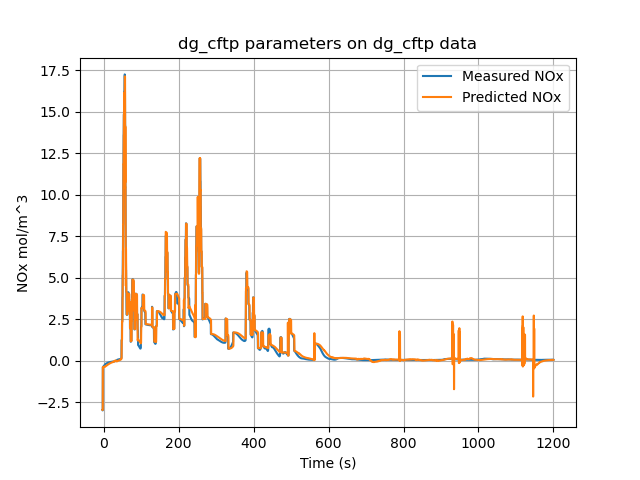
\includegraphics[width = \textwidth]{./figs/figs_new_mdl/dg_cftp_dg_cftp.png}
        \end{minipage}
        \begin{minipage}{0.3\textwidth}
                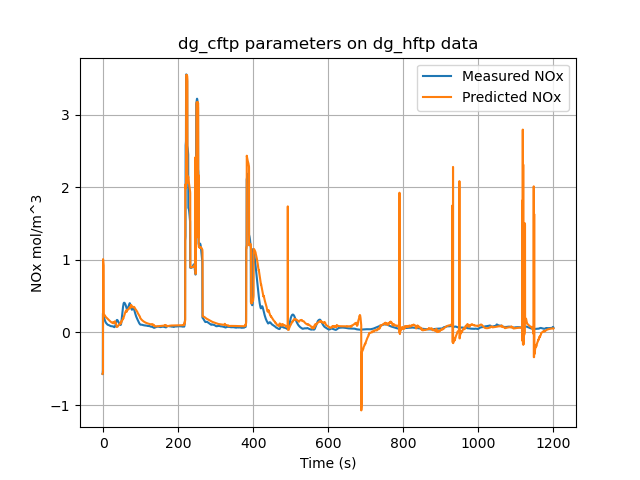
\includegraphics[width = \textwidth]{./figs/figs_new_mdl/dg_cftp_dg_hftp.png}
        \end{minipage}
        \begin{minipage}{0.3\textwidth}
                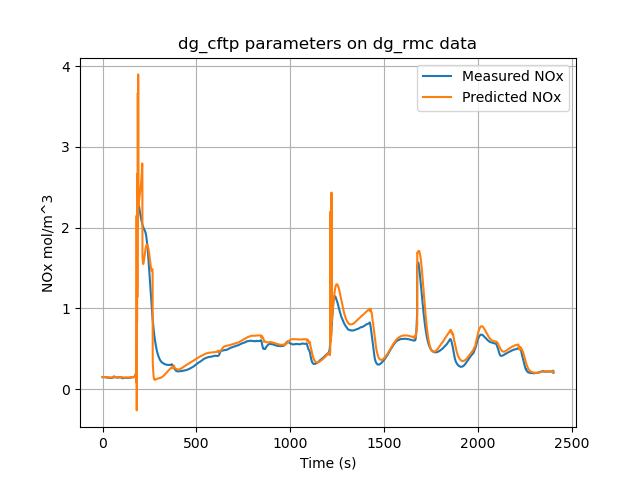
\includegraphics[width = \textwidth]{./figs/figs_new_mdl/dg_cftp_dg_rmc.png}
        \end{minipage}
        \caption{Cross validation using dg$\_$cftp parameter estimates}
\end{figure}

\begin{figure}[H]
        \begin{minipage}{0.3\textwidth}
                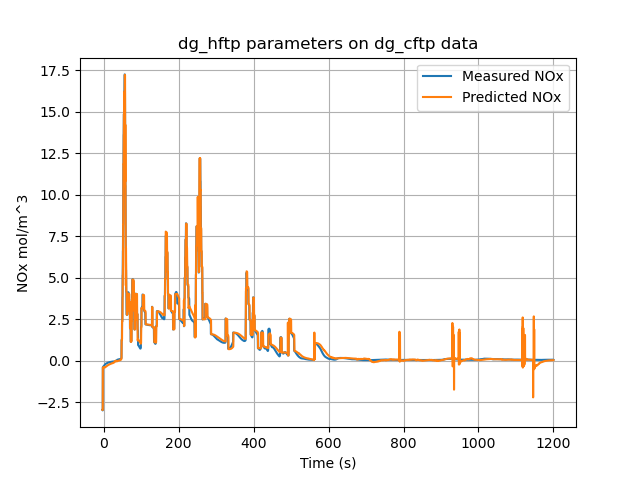
\includegraphics[width = \textwidth]{./figs/figs_new_mdl/dg_hftp_dg_cftp.png}
        \end{minipage}
        \begin{minipage}{0.3\textwidth}
                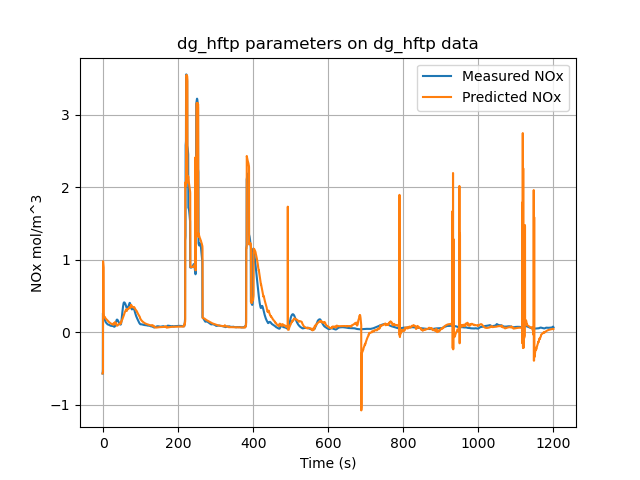
\includegraphics[width = \textwidth]{./figs/figs_new_mdl/dg_hftp_dg_hftp.png}
        \end{minipage}
        \begin{minipage}{0.3\textwidth}
                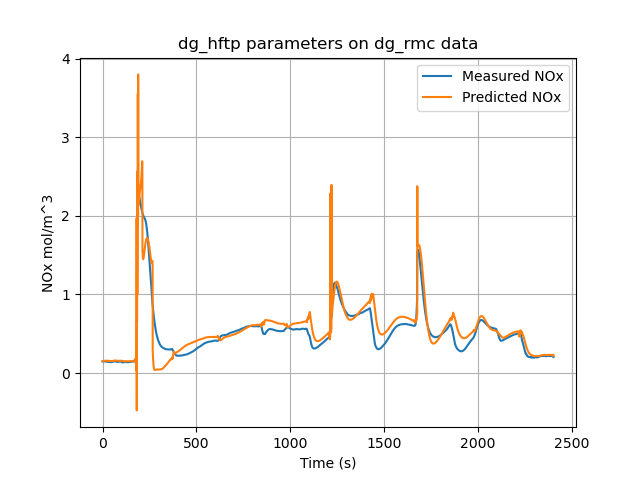
\includegraphics[width = \textwidth]{./figs/figs_new_mdl/dg_hftp_dg_rmc.png}
        \end{minipage}
        \caption{Cross validation using dg$\_$hftp parameter estimates}
\end{figure}

\begin{figure}[H]
        \begin{minipage}{0.3\textwidth}
                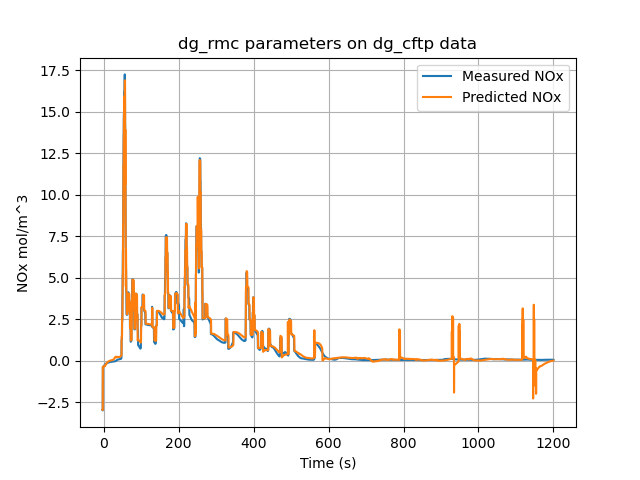
\includegraphics[width = \textwidth]{./figs/figs_new_mdl/dg_rmc_dg_cftp.png}
        \end{minipage}
        \begin{minipage}{0.3\textwidth}
                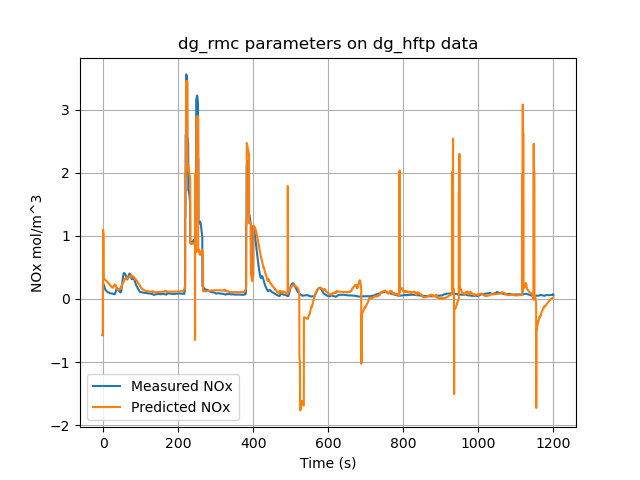
\includegraphics[width = \textwidth]{./figs/figs_new_mdl/dg_rmc_dg_hftp.png}
        \end{minipage}
        \begin{minipage}{0.3\textwidth}
                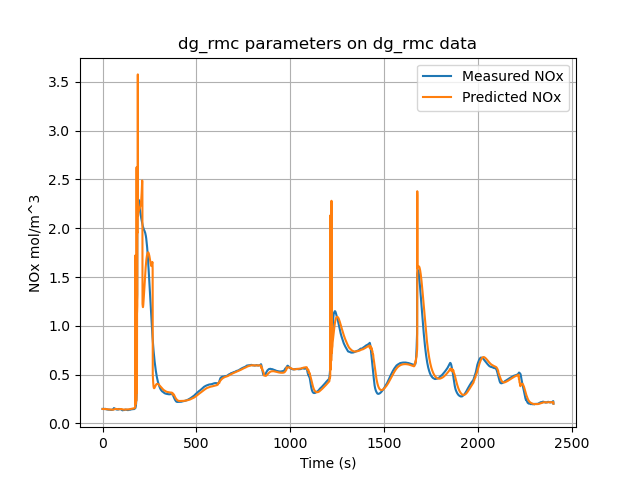
\includegraphics[width = \textwidth]{./figs/figs_new_mdl/dg_rmc_dg_rmc.png}
        \end{minipage}
        \caption{Cross validation using dg$\_$rmc parameter estimates}
\end{figure}


\subsection{Aged Test Data}

\begin{figure}[H]
        \begin{minipage}{0.3\textwidth}
                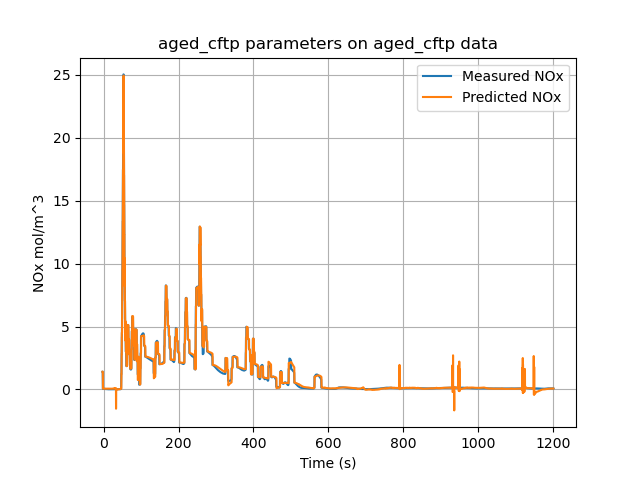
\includegraphics[width = \textwidth]{./figs/figs_new_mdl/aged_cftp_aged_cftp.png}
        \end{minipage}
        \begin{minipage}{0.3\textwidth}
                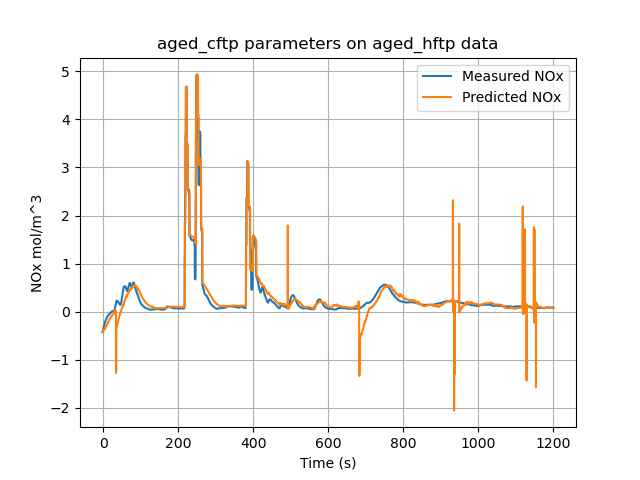
\includegraphics[width = \textwidth]{./figs/figs_new_mdl/aged_cftp_aged_hftp.png}
        \end{minipage}
        \begin{minipage}{0.3\textwidth}
                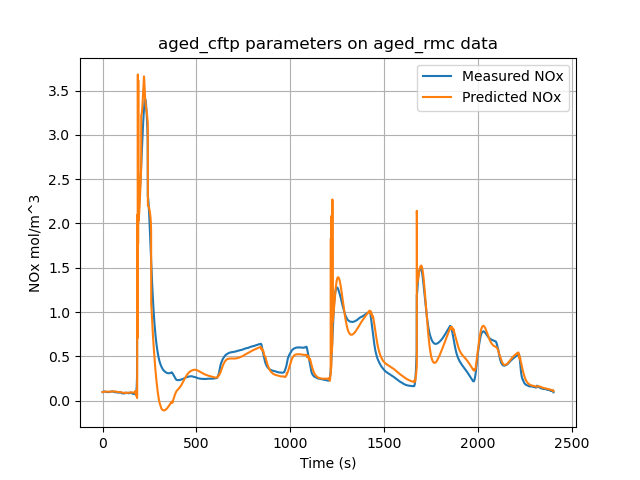
\includegraphics[width = \textwidth]{./figs/figs_new_mdl/aged_cftp_aged_rmc.png}
        \end{minipage}
        \caption{Cross validation using aged$\_$cftp parameter estimates}
\end{figure}

\begin{figure}[H]
        \begin{minipage}{0.3\textwidth}
                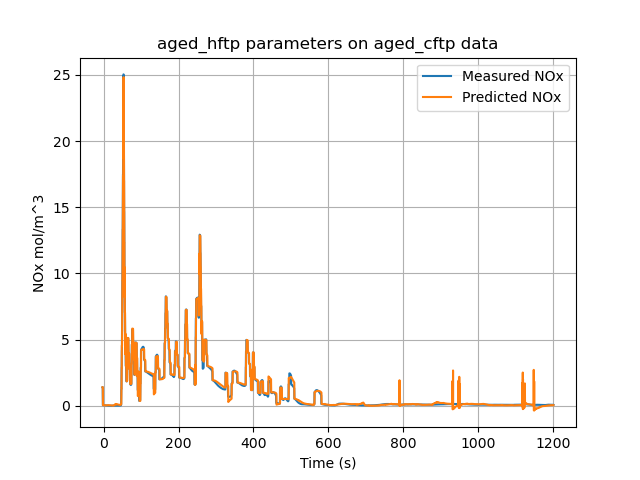
\includegraphics[width = \textwidth]{./figs/figs_new_mdl/aged_hftp_aged_cftp.png}
        \end{minipage}
        \begin{minipage}{0.3\textwidth}
                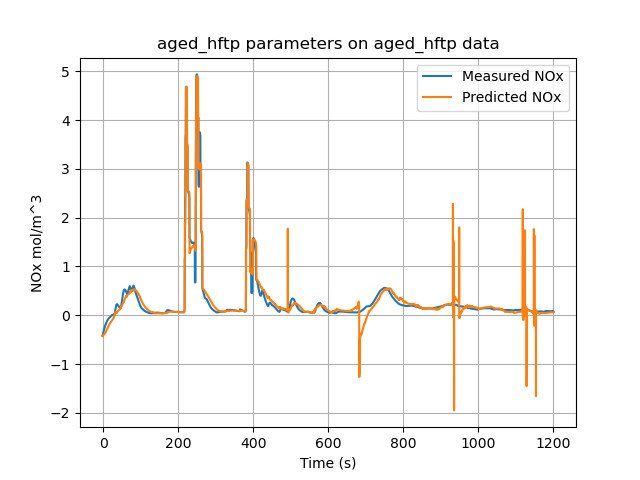
\includegraphics[width = \textwidth]{./figs/figs_new_mdl/aged_hftp_aged_hftp.png}
        \end{minipage}
        \begin{minipage}{0.3\textwidth}
                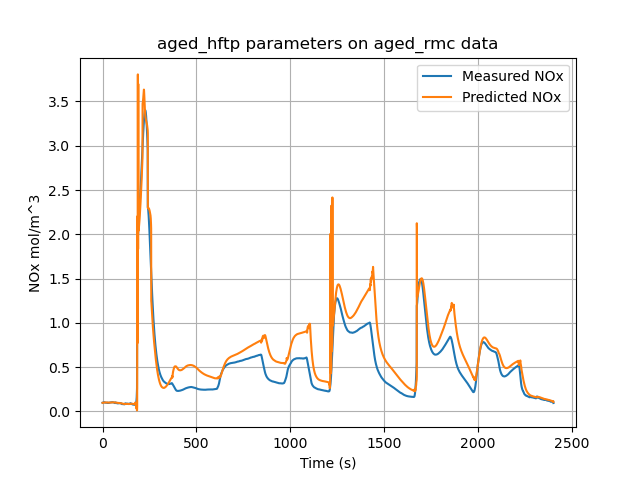
\includegraphics[width = \textwidth]{./figs/figs_new_mdl/aged_hftp_aged_rmc.png}
        \end{minipage}
        \caption{Cross validation using aged$\_$hftp parameter estimates}
\end{figure}

\begin{figure}[H]
        \begin{minipage}{0.3\textwidth}
                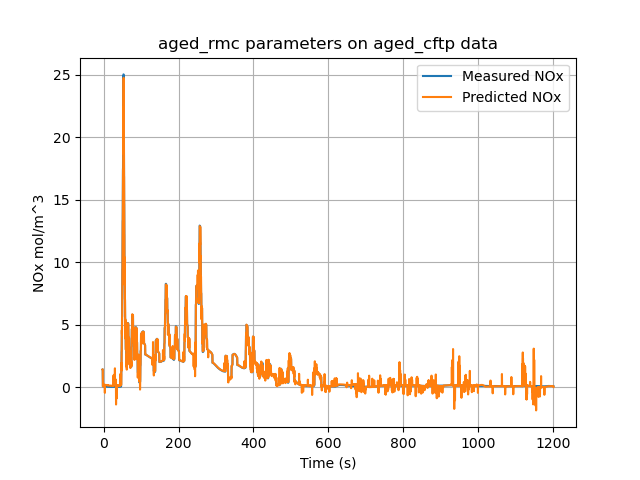
\includegraphics[width = \textwidth]{./figs/figs_new_mdl/aged_rmc_aged_cftp.png}
        \end{minipage}
        \begin{minipage}{0.3\textwidth}
                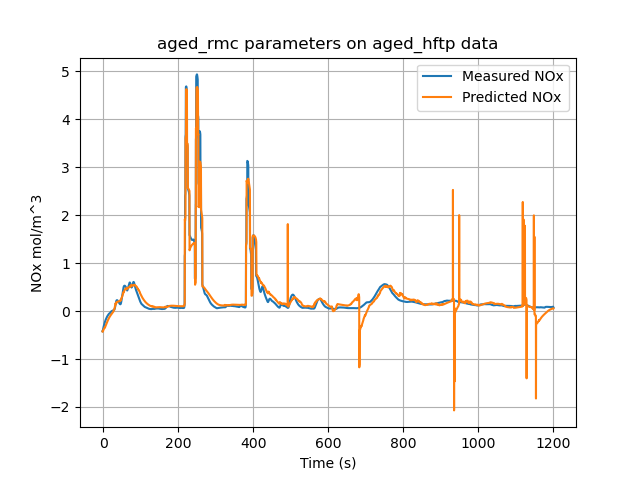
\includegraphics[width = \textwidth]{./figs/figs_new_mdl/aged_rmc_aged_hftp.png}
        \end{minipage}
        \begin{minipage}{0.3\textwidth}
                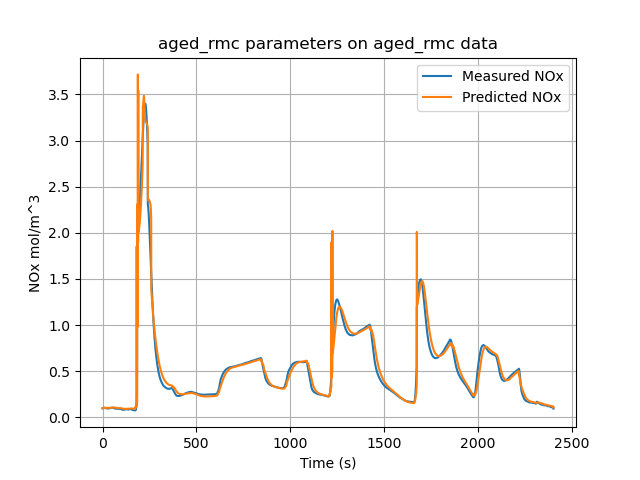
\includegraphics[width = \textwidth]{./figs/figs_new_mdl/aged_rmc_aged_rmc.png}
        \end{minipage}
        \caption{Cross validation using aged$\_$rmc parameter estimates}
\end{figure}


\subsection{Comparing Aged and Degreened parameter estimates}

\begin{figure}[H]
        \begin{minipage}{0.3\textwidth}
                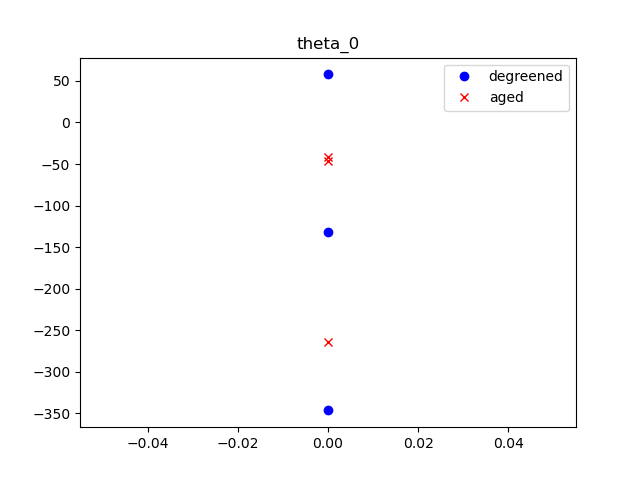
\includegraphics[width = \textwidth]{./figs/figs_new_mdl/theta_0.png}
        \end{minipage}
        \begin{minipage}{0.3\textwidth}
                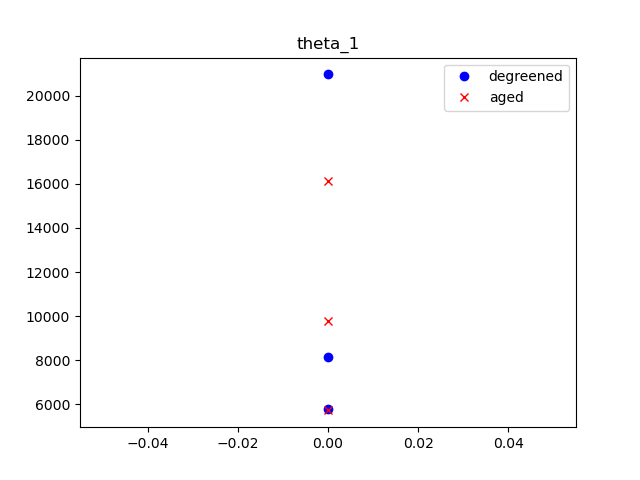
\includegraphics[width = \textwidth]{./figs/figs_new_mdl/theta_1.png}
        \end{minipage}
        \begin{minipage}{0.3\textwidth}
                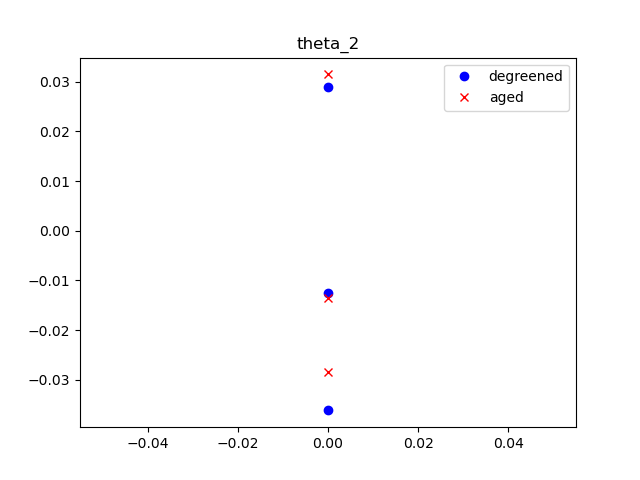
\includegraphics[width = \textwidth]{./figs/figs_new_mdl/theta_2.png}
        \end{minipage}
\end{figure}

\begin{figure}[H]
        \begin{minipage}{0.3\textwidth}
                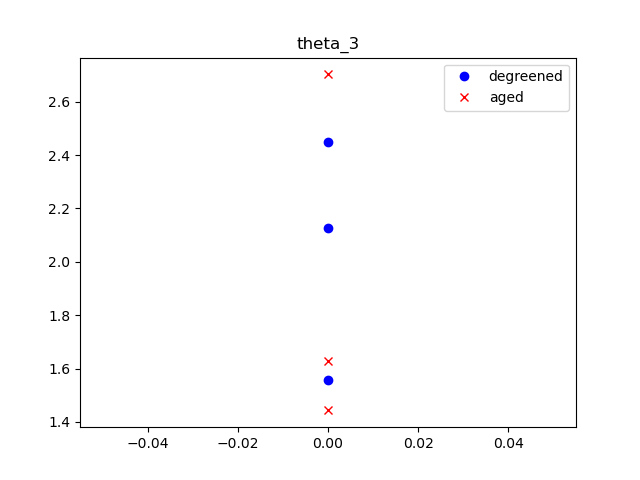
\includegraphics[width = \textwidth]{./figs/figs_new_mdl/theta_3.png}
        \end{minipage}
        \begin{minipage}{0.3\textwidth}
                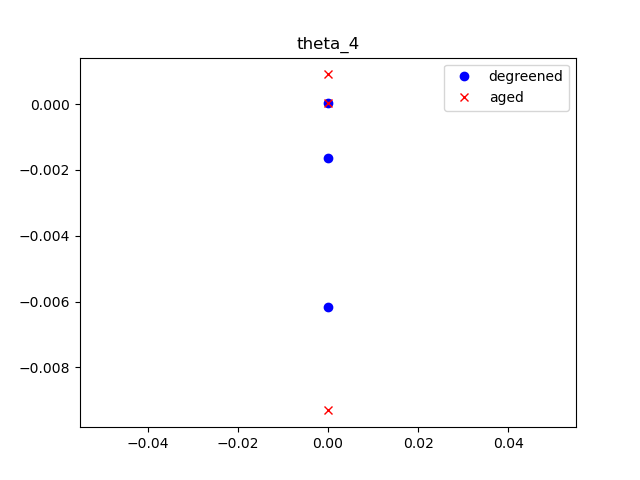
\includegraphics[width = \textwidth]{./figs/figs_new_mdl/theta_4.png}
        \end{minipage}
        \begin{minipage}{0.3\textwidth}
                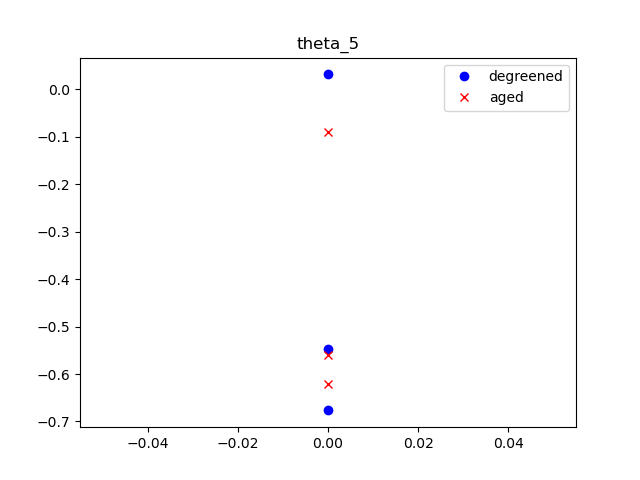
\includegraphics[width = \textwidth]{./figs/figs_new_mdl/theta_5.png}
        \end{minipage}
\end{figure}

\begin{figure}[H]
        \begin{minipage}{0.3\textwidth}
                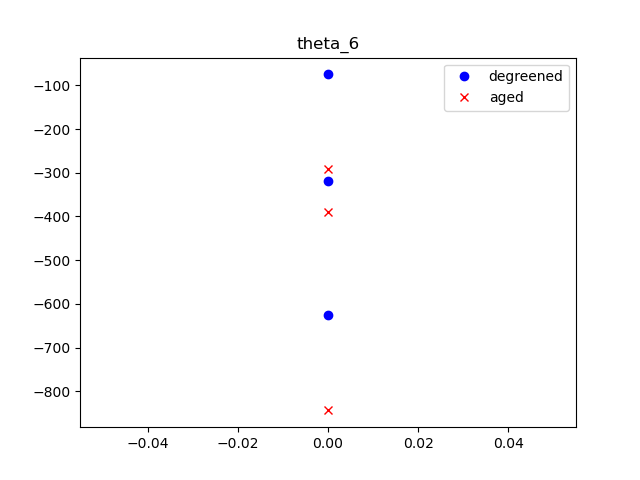
\includegraphics[width = \textwidth]{./figs/figs_new_mdl/theta_6.png}
        \end{minipage}
        \begin{minipage}{0.3\textwidth}
                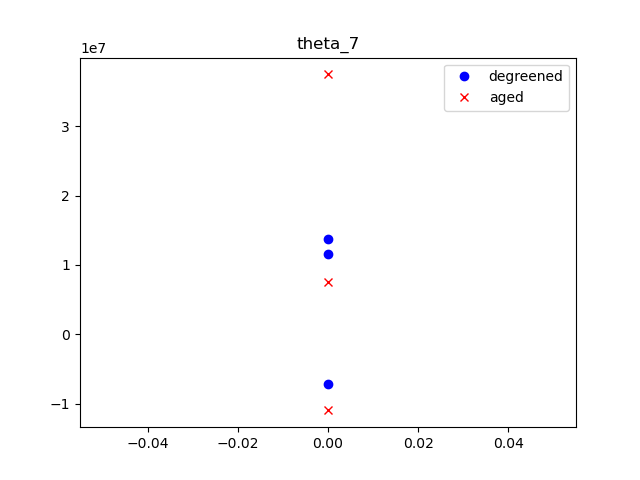
\includegraphics[width = \textwidth]{./figs/figs_new_mdl/theta_7.png}
        \end{minipage}
        \begin{minipage}{0.3\textwidth}
                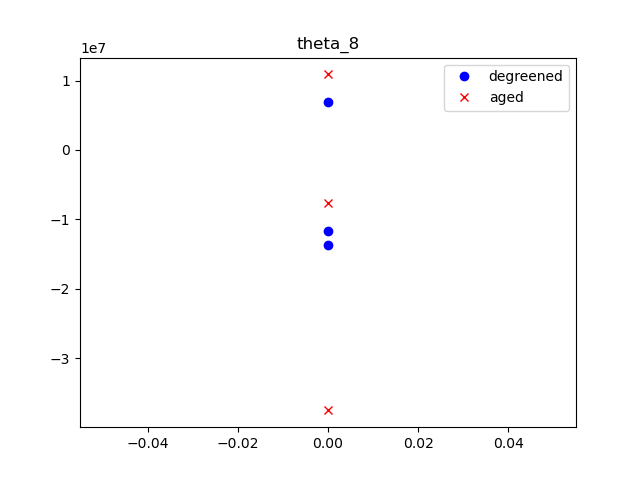
\includegraphics[width = \textwidth]{./figs/figs_new_mdl/theta_8.png}
        \end{minipage}
\end{figure}

\begin{figure}[H]
        \centering
        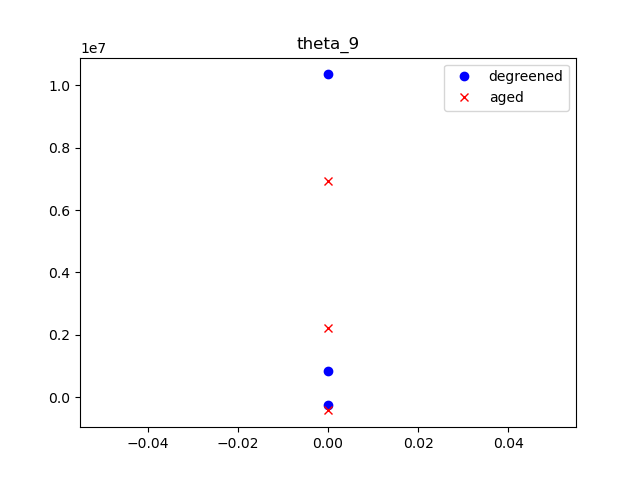
\includegraphics[width = 0.3\textwidth]{./figs/figs_new_mdl/theta_9.png}
\end{figure}

%\section{Remarks}
This work developed a uniquely identifiable parametric nonlinear model structure for SCR-ASC dynamics based on the first principles. The cross-validation results show the goodness of fit for the model. The parameters are not distinct with respect to the aging of the catalyst. The parametric structure is unique while the actual parameter and regression vectors can be tweaked based on models for rate constants, residence time and urea injection. This allows us to choose appropriate assumptions for the reduced order model for the process.

